\documentclass[12pt]{article}
\usepackage[utf8]{inputenc}
\usepackage{graphicx}
\usepackage{epigraph}
\usepackage{bbold}
\usepackage{amsmath}
\usepackage{mathtools}
\usepackage[hyperfootnotes=false]{hyperref}
\usepackage{tabularx}
\usepackage{siunitx}
\usepackage{float}
\usepackage{scrextend}
\usepackage{multicol}
\usepackage{lscape}
\usepackage{relsize}
\usepackage{tikz}
\usepackage{color}
\usepackage{listings}
\usepackage{setspace}
\usepackage[caption=false]{subfig}
\usepackage[symbol]{footmisc}
\usepackage[backend=biber,sorting=ynt,style=bath]{biblatex}
\usepackage[margin=1in]{geometry}
\usepackage[cache=false]{minted}
\assignrefcontextentries[]{*}
\renewcommand{\thefootnote}{\fnsymbol{footnote}}
\interfootnotelinepenalty=10000
\addbibresource{../lib.bib}
\setlength{\parindent}{0pt}
\DeclareMathOperator*{\argmax}{arg\,max}
\lstset{language=Java,breaklines,breakatwhitespace,basicstyle=\small}

\newenvironment{spaced}[1]
  {\begin{minipage}[c]{\textwidth}\vspace{#1}}
  {\end{minipage}}

\newenvironment{centrespaced}[2]
  {\begin{center}\begin{minipage}[c]{#1}\vspace{#2}}
  {\end{minipage}\end{center}}


\newcommand{\consultation}[1]{%
\thispagestyle{empty}
\begin{centrespaced}{0.8\textwidth}{0.4\textheight}
\ifnum #1 = 0
This dissertation may be made available for consultation within the University Library and may be photocopied or lent to other libraries for the purposes of consultation.
\else
This dissertation may not be consulted, photocopied or lent to other libraries without the permission of the author for #1 
\ifnum #1 = 1
year
\else
years
\fi
from the date of submission of the dissertation.
\fi
\end{centrespaced}
}

\newcommand{\declaration}[2]{
  \thispagestyle{empty}
  \begin{spaced}{4em}
    \begin{center}
      \LARGE\textbf{#1}
    \end{center}
  \end{spaced}
  \begin{spaced}{3em}
    \begin{center}
      Submitted by: #2
    \end{center}
  \end{spaced}
  \begin{centrespaced}{0.8\textwidth}{0.1\textheight}
    \section*{Copyright}
Attention is drawn to the fact that copyright of this dissertation rests with its author. The Intellectual Property Rights of the products produced as part of the project belong to the author unless otherwise specified below, in accordance with the University of Bath's policy on intellectual property (see \url{https://www.bath.ac.uk/publications/university-ordinances/attachments/Ordinances_1_October_2020.pdf}).

This copy of the dissertation has been supplied on condition that anyone who consults it is understood to recognise that its copyright rests with its author and that no quotation from the dissertation and no information derived from it may be published without the prior written consent of the author.
    \section*{Declaration}
This dissertation is submitted to the University of Bath in accordance with the requirements of the degree of Bachelor of Science in the Department of Computer Science. No portion of the work in this dissertation has been submitted in support of an application for any other degree or qualification of this or any other university or institution of learning. Except where specifically acknowledged, it is the work of the author.
  \end{centrespaced}
  }


\title{\bf Zero-Knowledge Approaches to Tetris}
\author{Tyler Christie}
\date{Bachelor of Science in Computer Science\\ 
                                 % E.g.: Bachelor of Science in Computer Science
                                 %       Master of Science in Data Science
      The University of Bath\\
      2021-22}

\begin{document}

\hypersetup{pageanchor=false}

\setcounter{page}{0}
\pagenumbering{roman}

\maketitle
\newpage

\consultation{0}
\newpage

\declaration{Zero-Knowledge Approaches to Tetris}{Tyler Christie}
\newpage

\hypersetup{pageanchor=true}

\abstract
We study the capabilities of reinforcement learning approaches in the game of Tetris without the utilisation of prior human knowledge. Tetris is a complex environment with a state space so large that it cannot be tabulated, and not every state can be visited. We examine the effects of state representation, reward structure and exploration strategy on agent performance in an effort to maximise efficient exploration and exploitation of agent-acquired domain knowledge using Proximal Policy Optimisation and Deep-Q Networks. Our findings indicate that, with appropriate network architecture, making a longer `history' of states available to the agent improves performance. Secondly, a reward structure based on the original Tetris score acheives the best performance for both PPO and DQN, but that other reward structures show more promise for continued improvement and should be explored further. Finally, we show that exploration via intrinsic rewards for information gain significantly improves the performance of PPO, and similarly, exploration via bootstrapped value network sampling for DQN has the same effect. 
\newpage

\tableofcontents
\newpage

\listoffigures
\newpage

\listoftables
\newpage

\section*{Acknowledgements}

Whilst this may be an individual project, no man is an island, and this wouldn't have been possible without the support from those around me. I'd like to thank my parents for their endless emotional support and proofreading, without which I'm sure I would have thrown in the towel. Thank you to my supervisor Matt Hewitt for his expert guidance and feedback, who selflessly endured hour-long meetings full of my ramblings. Finally, I'd like to thank Tom Haines, for his quick and helpful resolution of technical issues with the university compute cluster. 

\newpage
\setcounter{page}{1}
\pagenumbering{arabic}

\section{Introduction}
\epigraph{``Reinforcement learning is the learning of a mapping from situations to actions so as to
maximize a scalar reward or reinforcement signal.''}{\textit{Richard S. Sutton}}  
Richard S. Sutton, who can be considered an authoritative voice in the field of Reinforcement Learning (hereinafter out referred to as RL), accurately summarizes the essence of this domain in the above quote. The learning agent in a RL environment produces an output signal in the form of an action, and receives an input signal in the form of a reward.
Trial-and-error search; namely, the balance between exploration of unknowns and exploitation of current knowledge, and the concept of delayed reward can be considered to be two of the
distinguishing features when compared to other machine learning paradigms (those of supervised and unsupervised learning) \autocite{Sutton2012-uz}.\\\newline 
Exploration versus exploitation is an interesting trade-off; if an agent explores too much, it risks spending too little time exploiting what it has learnt to its advantage. If it explores too little, the agent risks missing out on the aquisition of the optimal strategy.
\\\newline Every reinforcement learning method is essentially trying to find a solution to the following equation and variations of it \autocite{10.5555/3312046}:
\begin{equation}\label{sve}
        V_{\pi}(s) = E_\pi[R(s,a) + \gamma V(s')]=\underset{a}{\Sigma}\pi(a|s)\underset{s'\in S}{\Sigma}\underset{r\in R}{\Sigma}p(s',r|s,a)(r+\gamma V_\pi(s'))
\end{equation}
The State-Value function assigns an expected value $E$ following a policy $\pi$ by adding the reward of taking an action from policy $\pi$ in the current state to the discounted (where $\gamma$ is our discount factor) reward of the next state. Throughout the literature review we will unpack and discuss this equation.\\\newline
It is worth defining at this point a few key terms of the domain:
\paragraph{Agent} The aspect of the problem under direct control; the learning and acting entity that attempts to maximise the reward it receives.
\paragraph{Action} A method of the agent through which it interacts with and changes its environment.
\paragraph{Discount Factor $\gamma$} A factor multiplying the future reward; a smaller discount factor signifies future rewards are less important, and vice versa. 
\paragraph{Environment} Everything that is not under direct sovereignty of the agent; everything the agent can interact with. 
\paragraph{Episode} The sequence of states between an initial state and a terminal state; a play-through.\\\newline
It is hard to find a concrete definition of these terms, however all the literature cited in this review uses these terms in the same way. Other terminology will be introduced as required. 
\\\newline Tetris is an important benchmark for the field of reinforcement learning, as it has a complex state space such that virtually no situation is encountered twice, and necessitates medium-to-long-term planning. \\\newline
The mechanics of the game are simple; it is played on a two-dimensional grid, typically 20x10. The grid begins in an empty state, and slowly fills up as tetriminos - shapes consisting of four squares - fall from the top. The player has the ability to change the column in which the shape drops, and rotate the shape as it falls. Despite this apparently simple concept, the game has been proven to be NP-complete \autocite{demaine2003tetris}, although it has also been shown that there are sequences that will definitively end a game \autocite{burgiel1997lose}. \\\newline
Furthermore, no efficient learning algorithm has been developed that works with Tetris. Current literature utilises hand-crafted feature sets and complex, computation heavy evolutionary algorithms to achieve good performance, and as of yet there has been no successful pure reinforcement learning attempts. As discussed later, solving the game of Tetris could potentially lead to breakthroughs in other areas of reinforcement learning research, and as such, this paper seeks to further explore the zero-knowledge approach to Tetris by applying PPO and DQN algorithms, and by shaping reward, state space and exploration stategy.  \\\newline
Section \ref{litrev} of this paper covers the core concepts in RL required to understand the hypotheses we propose in our experiments. Section \ref{mltetty} covers previous applications of machine learning to Tetris. Section \ref{design} describes our experiment setup and Section \ref{algo} outlines the code that implements this. Section \ref{resultsanal} covers the results of our experiments and discussion, Section \ref{limits} covers the limitations of the scope of this research alongside difficulties encountered, and Section \ref{conclusion} concludes the paper. 
\newpage
\section{Literature Survey and Review}\label{litrev}
Reinforcement Learning has a short but active history with two main threads of origin; animal learning psychology and optimal control theory. Whilst these two fields were largely independent of each other originally, they eventually converged to form the field of reinforcement learning. 
\\\newline As noted by \textcite{watkins1989learning}, there were mainly two types of experimental procedure used in animal learning studies; instrumental learning and classical (or Pavlovian) learning. The former entails reinforcement stimuli depending on the action of the animal, whereas the latter consists of reinforcers contingent on an event, regardless of the animals response. 
Omitting the detail Watkins goes into in his thesis, the essence is that the function of instrumental learning is to find the optimal behaviour given certain criteria; a performance critereon which allows us to judge the efficiency of our behaviour - in an animal this is decided internally, and in reinforcement learning this is our reward signal $r$.
\\\newline Sutton \autocite{Sutton2012-uz} describes the other origin of reinforcement learning; that of the domain of optimal control problems. The term `optimal control' describes the set of problems concerning the minimisation or maximisation of some measure of a dynamic systems behaviour over time. This eventually lead to the derivation of the functional equation now known as the Bellman equation (Equation \ref{sve}), and the class of algorithms for solving this equation, now known as `dynamic programming' (although the field of dynamic programming extends far beyond solving Bellman equations). Bellman at this time also introduced Markov Decision Processes (MDPs) \autocite{bellman1957markovian}, discussed in Section \ref{markov}, all of which became the major corner stones underlying the modern field of reinforcement learning.
\subsection{Markov Decision Processes (MDPs)}\label{markov}
Markov Decision Processes are a critical tool for modeling the interaction of an agent and its environment, and as such are an indispensable feature of the field of reinforcement learning and machine learning in general.\\\newline
A sequence of random variables $X_1,X_2,...X_n$ is a Markov chain if the conditional distribution of $X_{n+1}$ given $X_1,X_2,...X_n$, depends on $X_n$ only \autocite{brooks2011handbook}. That is, if every element in the sequence depends on the previous element only to determine its probability distribution.
A system can be considered to have the Markov property if it satisfies the definition of a Markov chain \autocite{1976Ttos}. As a probability it can be denoted: 
\begin{equation}
    P[S_{t+1} | S_t] = P[S_{t+1} | S_1, S_2, ...,S_t]
\end{equation}
Which simply states that the probability of a system entering state $S_{t+1}$ given $S_t$ is the same as the probability given every state up to $S_t$.
With this set of states $S$ satisfying the Markov property, we can now construct a Markov Decision Process, which is formally defined by \textcite{thomas2015notation} as a tuple $(S,A,\mathcal{R},P,R,d_0,\gamma)$ where:
\begin{itemize}
 \item   $t$ denotes the time step, where $t>\mathbb{N}_0$
 \item$S$ denotes the set of possible states an agent can be in, and $s$ denotes an individual state in the set $S$.
 \item $A$ denotes the set of possible actions of an agent \autocite{haggstrom2002finite}
 \item$\mathcal{R}\subseteq\mathbb{R}$ denotes the set of possible rewards an agent can receive
 \item$P:S\bigtimes A \bigtimes S \rightarrow [0,1]$ is the transition function 
 \item$R$ denotes the reward function 
 \item$d_0$ denotes the initial state distribution 
 \item$\gamma\in [0,1]$ denotes the reward discount factor
\end{itemize}
The elements of transition function $P$ are called transition probabilties \autocite{haggstrom2002finite}. The transition probability $P_{i,j}$ is the conditional probability of being in state $s_j$ at time $t+1$ given that we are in state $s_i$ at time $t$ \autocite{haggstrom2002finite}. The conditional probability of $X_{n+1}$ given $X_n$ (here we use the notation of a Markov chain, but recall that the states $S$ observe the Markov property and therefore form a Markov chain) is the same for all $t$ \autocite{haggstrom2002finite}. This property is known as time homogeneity, and in general it is assumed that all Markov chains observe this property \autocite{haggstrom2002finite}.\\\newline
To exemplify the use of an MDP, here is a well-known learning problem:
\subsection{The Recycling Robot}
A robot collects rubbish around an office. At any given time, the robot can either (a) search for rubbish (b) wait or (c) return to it's charging station. The robot is either in a $high$ state or $low$ state, indicating its battery level. The reward it receives is the number of items of rubbish it collects. The MDP can be represented as the figure seen below: 
\begin{figure}[H]
    \begin{center}
        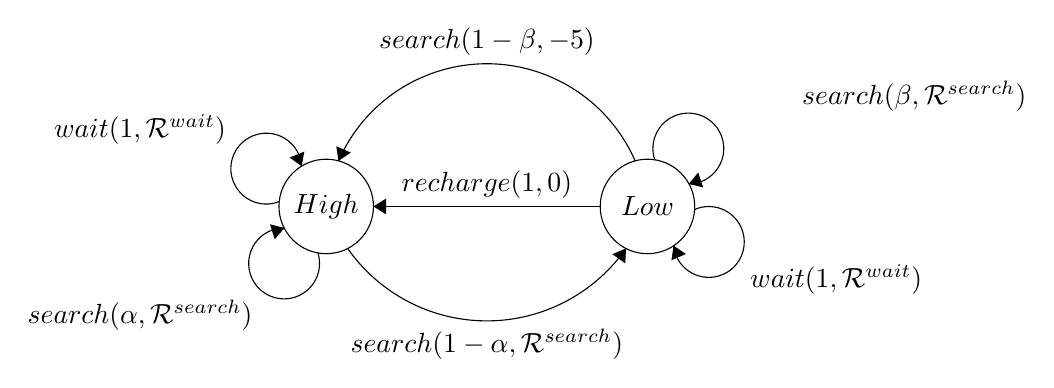
\begin{tikzpicture}[scale=0.2]
        \tikzstyle{every node}+=[inner sep=0pt]
        \draw [black] (27.1,-29.4) circle (3);
        \draw (27.1,-29.4) node {$High$};
        \draw [black] (47.5,-29.4) circle (3);
        \draw (47.5,-29.4) node {$Low$};
        \draw [black] (47.965,-26.448) arc (198.78241:-89.21759:2.25);
        \draw (64.44,-23.39) node [above] {$search(\beta,\mathcal{R}^{search})$};
        \fill [black] (50.13,-27.97) -- (51.04,-28.19) -- (50.72,-27.24);
        \draw [black] (44.5,-29.4) -- (30.1,-29.4);
        \fill [black] (30.1,-29.4) -- (30.9,-29.9) -- (30.9,-28.9);
        \draw (37.3,-28.9) node [above] {$recharge(1,0)$};
        \draw [black] (50.482,-29.598) arc (113.93142:-174.06858:2.25);
        \draw (53.99,-34.02) node [right] {$wait(1,\mathcal{R}^{wait})$};
        \fill [black] (49.16,-31.89) -- (49.02,-32.82) -- (49.94,-32.42);
        \draw [black] (27.881,-26.514) arc (156.49615:23.50385:10.272);
        \fill [black] (27.88,-26.51) -- (28.66,-25.98) -- (27.74,-25.58);
        \draw (37.3,-19.84) node [above] {$search(1-\beta,-5)$};
        \draw [black] (46.141,-32.064) arc (-34.99195:-145.00805:10.792);
        \fill [black] (46.14,-32.06) -- (45.27,-32.43) -- (46.09,-33.01);
        \draw (37.3,-37.17) node [below] {$search(1-\alpha,\mathcal{R}^{search})$};
        \draw [black] (26.571,-32.341) arc (17.53077:-270.46923:2.25);
        \draw (15.28,-35.33) node [below] {$search(\alpha,\mathcal{R}^{search})$};
        \fill [black] (24.44,-30.77) -- (23.53,-30.53) -- (23.83,-31.49);
        \draw [black] (24.128,-29.087) arc (291.72436:3.72436:2.25);
        \draw (20.77,-24.5) node [left] {$wait(1,\mathcal{R}^{wait})$};
        \fill [black] (25.54,-26.85) -- (25.71,-25.92) -- (24.78,-26.29);
        \end{tikzpicture}
        \end{center}
        \caption{an MDP of the recycling robot problem}
        \label{recrob}
\end{figure}
~\\On each transition, the label reads $action(transition\_probability,reward)$. A $search$ completed from the high state returns the robot to the $high$ state with the probability $\alpha$ and to the $low$ state with probability $1-\alpha$. A $search$ from the $low$ state returns the robot to the $low$ state with probability $\beta$ and depletes the battery with probability $1-\beta$. If the battery is depleted, the robot must be manually returned to the charging point, thus the reward is negative (here I have put -5 but the amount is not significant, just enough so that the robot considers it worthwhile to avoid this outcome). For the robot to operate effectively, we must have $\mathcal{R}^{search}>\mathcal{R}^{wait}$, else the robot will simply do nothing. Formally, the MDP above can be considered as: 
\begin{itemize}
    \item $S = \{high,low\}$
    \item $A = \{search,wait,recharge\}$
    \item $\mathcal{R} = \{\mathcal{R}^{search},\mathcal{R}^{wait},0,-5\}$  
\end{itemize}
And the transition function:
\renewcommand{\arraystretch}{1.2}
\begin{figure}[H]
    \centering
    \begin{tabular}{|c|c|c|c|c|}\hline
        $s=s^t$ & $A$ & $s=s^{t+1}$ & $P$ & $\mathcal{R}$ \\\hline 
        high & search & high & $\alpha$ & $\mathcal{R}^{search}$ \\\hline
        high & search & low & $1-\alpha$ & $\mathcal{R}^{search}$ \\\hline   
        low & search & low & $\beta$ & $\mathcal{R}^{search}$ \\\hline   
        low & search & high & $1-\beta$ & $-5$ \\\hline   
        high & wait & high & $1$ & $\mathcal{R}^{wait}$ \\\hline   
        high & wait & low & $0$ & $\mathcal{R}^{wait}$ \\\hline   
        low & wait & low & $1$ & $\mathcal{R}^{wait}$ \\\hline   
        low & wait & high & $0$ & $\mathcal{R}^{wait}$ \\\hline   
        high & recharge & high & $1$ & $0$ \\\hline   
        high & recharge & low & $0$ & $0$ \\\hline 
        low & recharge & high & $1$ & $0$ \\\hline   
        low & recharge & low & $0$ & $0$ \\\hline       
    \end{tabular}
    \caption{Transition Probabilities and Rewards}
\end{figure}
Most learning problems (although there are exceptions) can be modelled as MDPs, including the game of Tetris. For problems with continous values, once they are quantized again they can be represented as an MDP, or as a continuous MDP.
\subsection{Neural Networks}\label{networks}
Neural Networks have gone in and out of fashion since their conception in 1943 by \textcite{mcculloch1943logical}, enjoying a resurgence in the 1980s, in part due to \textcite{werbos1974beyond} backpropagation algorithm, and once again falling back into obscurity before an uptake in recent decades through the veil of `deep learning'.\\\newline
Artificial Neural Networks (ANNs), usually shortened to Neural Networks (NNs) are computational systems modelled after the animal brain. The field of NNs has evolved independently many separate times in many different fields, so it remains difficult to reach consensus on a canonical formalization. \textcite{haykin2010neural} offers the following definition: \\\newline
\begin{addmargin}[2em]{0em}% 1em left, 2em right
    \textit{``A neural network is a massively parallel distributed processor made up of simple processing
    units that has a natural propensity for storing experiential knowledge and making it available
    for use. It resembles the brain in two respects:}
    \begin{enumerate}
        \item \textit{Knowledge is acquired by the network from its environment through a learning process.}
        \item \textit{Interneuron connection strengths, known as synaptic weights, are used to store the acquired knowledge.''}
    \end{enumerate}
\end{addmargin}
Note that this is a very high level interpretation of a neural network and we will expand this definition later. This fits in line with our previous idea of the neural network modelling itself after the brain. The simple processing units mentioned in this definition are our `neurons', and their connections the `synapses'. The purpose of modelling a brain, intuitively, is to be able to emulate functions of the brain; namely problem-solving and pattern recognition. Pattern recognition allows us to generalize - from data we have seen to data we have not previously encountered. This is the primary use of neural networks; to provide function approximations for complex, intractable problems. 
 We can start by formalizing the idea of the neuron: \\\newline
The simplest and earliest model of a neuron is known as the McCulloch–Pitts Model \autocite{mcculloch1943logical}, defined in their 1943 paper. It consists of:
\begin{enumerate}
    \item A set of input $synapses$, each of which have a weight which signals the importance of this synapse.
    \item A combiner function for summing these input signals.
    \item An activation function, which decides whether a neuron fires or not.
\end{enumerate} 
\begin{figure}[H]
    \centering
    \includegraphics[scale=0.8]{2.png}
    \caption{A McCulloch-Pitts Neuron }
    \label{neuron}
\end{figure}
Figure \ref{neuron} illustrates a basic neuron of a neural network. We can define our combiner or aggregator function as : 
\begin{equation}
    u_k = \sum\limits_{i=0}^{i=n}w_ix_i
\end{equation}
Which simply sums the input signals multiplied by their weight. Notice that the sum of the aggregator function iterates from 0 through n, however the input nodes in Figure \ref{neuron} range from 1 to n. This is to account for $w_0$, the bias of our network (the input $x_0$ is fixed at 1). We can think of the bias as the $c$ if we compare the function of a neuron to the straight line equation $y = mx+c$. Our output $y_k$ is defined as:
\begin{equation}
    y_k = \phi(u_k)
\end{equation} 
Simply our activation function applied to our input (from the aggregator function). \\\newline
There are many different activation functions. Referring back to our definition of a neural network, we know that the purpose of NNs is to approximate functions, which fundamentally come in two different formats; linear and non-linear. If we have no activation function; that is, if the signal passes through neurons unchanged, then the network effectively becomes a linear regression model, only capable of solving linear equations. To solve any more complex problem, we need to introduce non-linearity; an activation function. The type of activation function we choose depends on the problem we are trying to model. Here are a few of the most basic activation functions:
\paragraph{Threshold Function} A boolean function that distinguishes ranges of values above a certain `threshold' \autocite{dodge2003the}. This satisfies the $all-or-none$ property of neurons as describes in McCulloch's and Pitt's paper \autocite{mcculloch1943logical}; nerve cells will give the maximum response or none at all. This could be used for yes-no type problems, although not multi-class classification problems as by its very nature it can only distinguish between two classes. 
\paragraph{Sigmoid Function} Another commonly used activation function, otherwise known as the standard logistic function in the field of ANNs \autocite{10.1007/3-540-59497-3_175}; It provides a return value in the range 0 to 1, with larger inputs resulting in a value closer to 1, thus being a useful activation function for problems requiring a probability as output. It is defined as follows \autocite{10.1007/3-540-59497-3_175}:
\begin{equation}
    S(x) = \frac{1}{1+e^{-ax}}
\end{equation}
Where $a$ is an optional \textit{slope parameter} that dictates the gradient. Sometimes, stochastic models of neurons can be useful:
\begin{equation}
    S(x) = \frac{1}{1+e^{-x/T}}
\end{equation}
Where $T$ is a `temperature' that represents noise (randomness) in the network \autocite{haykin2010neural, Keeler1712}. This noise level parameter is an emulation of the actual noise that occurs in a biological neural network \autocite{Keeler1712}. This is where we depart from the simple McCulloch–Pitts neuron model;  whilst the McCulloch–Pitts model was deterministic in its output, for cases where we want to model partially random behaviour, for example if we wanted to emulate human responses to some stimuli like the Rubin's vase \autocite{rubin1915synsoplevede}, non-deterministic behaviour is required. Admittedly the applications for stochastic neural nets are few and far between, although the use of Bayesian Neural Networks is enjoying a surge in uptake in recent years, and features in one of our experiments.
\\
\paragraph{Rectified Linear Unit (ReLU)}
ReLU is by the far the most commonly used activiation function in modern research due to being easily differentiable and thus easily computed, and having good gradient propagation properties \autocite{pmlr-v15-glorot11a} (i.e. fewer vanishing gradient problems compared to sigmoidal functions) amongst other advantages. It is defined as \autocite{DBLP:conf/icml/NairH10}:
\begin{equation}
    f(x) = max(0,x)
\end{equation}
Aside from the listed benefits which have seen ReLU functions made commonplace today, there is evidence for strong biological motivations. Whilst neural nets nowadays are a far stretch from their biological roots, there is evidence that the activation pattern of ReLU is very similar to actual neuron activation functions, more so than sigmoid or tanh functions \autocite{pmlr-v15-glorot11a}.\\\newline
Having covered the basic elements of a neuron, we can now discuss NN architectures. While there are dozens of types of NN architectures, there are two basic fundamental types.
\subsubsection{Feedforward Networks}\label{ffnets}
Feedforward networks were the first type of ANN, the simplest and earliest of which was Rosenblatt's Perceptron \autocite{rosenblatt1958perceptron}; a single neuron (of the McCulloch-Pitts model) neural network with the aforementioned threshold function (more specifically the Heaviside step function \autocite{8093960}) as its activation function. Feedforward networks are named as such because information in the input layer is `fed forward' through all the layers until reaching the output layer, without any loops or feedback connections (i.e. outputs from neurons are not fed back into the neural network). The simplest type of feedforward network has no hidden layers, and can be seen below:
\begin{figure}[H]
    \centering
    \includegraphics[scale=0.7]{3.png}
    \caption{Single-Layered Feedforward Network}
    \label{singlelayer}
\end{figure}
Single-Layered Networks as seen in Figure \ref{singlelayer} consist of a single input layer and a single output layer; it is considered single-layered as there is only a single computational layer (no computation is performed in the input layer). Data flows directly from the left to the right, ergo `feedforward'. \\\newline Note here that since every neuron in the output layer is connected to every node in the input layer, the network is said to be fully connected, or densely connected \autocite{haykin2010neural}. Similarly, if a layer is fully connected to the previous layer, this is a fully connected layer. Fully connected layers are what we generally see in neural networks, and they are for general purpose learning; no neuron within a layer is differentiated from one another. As a consequence however, the linear combination each neuron must perform of its inputs is larger, and as such the computational requirements are heavier. The inverse of this, namely partially connected layers, is generally only used in a convolutional layer of a CNN (Convolutional Neural Network) as these partial connections are particularly useful for feature recognition in image processing tasks \autocite{8308186}.\\\newline
Certain problems may require multiple transformations of the data to reach a desired output. Crudely speaking, hidden layers allow us to solve `higher-order statistical problems' \autocite{ChurchlandPatriciaS2016CO}.\\\newline
With a single computational layer, we are only able to answer questions such as `Does A correlate with B?'; that is, questions that can be solved with a single non-linear function application. For questions of any more complexity than this, such as `How do A,B,C,D correlate?', hidden layers give the network the `global perspective' to be able to answer these \autocite{ChurchlandPatriciaS2016CO}.\\\newline
To elucidate this matter further with an example; suppose that we want to use a NN to calulate a logical XOR of our set of inputs, and allow that activation functions in our network can only be simple logical operators. Using simple operators, we cannot compute the XOR of a set of inputs in a single layer, however if we allow for an additional hidden layer, this computation becomes possible. Assuming an interpretation of XOR as below:
\begin{figure}[H]
    \[ f(\vec{x}) = \begin{cases} 
        1 & \text{\textit{iff} one or more, but not all, of $x_1\dots x_n \in \vec{x}$ is 1} \\
        0 & \text{otherwise}
     \end{cases}
  \]
\end{figure}
 As opposed to the more standard two input version. See the figure below for a neural net to compute this function: 
\begin{figure}[H]
    \centering
    \includegraphics[scale=0.8]{4.png}
    \caption{Multi-Layered Feedforward Neural Network}
    \label{multilayer}
\end{figure}
Figure \ref{multilayer} shows us that adding a hidden layer enables us to transform our input in a helpful way for our output; with OR and NAND as the activation functions of the respective hidden layer neurons, our output layer is able to make use of 'higher-order' statistics that would not be available in a single-layer network.\\\newline
Whereas input and output layer neuron counts are easily determined; the number of input nodes must match the shape of the data, and the number of output nodes is determined by the answer desired, configuration of hidden layers is a highly contentious subject with no academic consensus on any formal rules for determining the parameters of hidden layers (such as number of nodes and number of layers). However there are some general rules of thumb to go by: few problems benefit from more than one hidden layer, and the number of nodes is almost always between your input size and your output size \autocite{Q+A_SAS}. This is further supported by the work of \textcite{cybenko1989approximations} and \textcite{hornik1991approximation}, who jointly proved the universal approximation theorem, which states that a feed-forward neural network with a single hidden layer and a finite number of neurons can approximate any continuous function (note however, that this does not imply that it would be \textit{easy} for the NN to actually learn something). Techniques are available, namely pruning algorithms, for optimizing network structure, a in-depth survey of which can be found by \textcite{248452}. 
\\\newline In light of these new concepts, we can now fully understand a more formal definition of a neural network, one which is generally accepted in the field and has been cited or paraphrased many times \autocite{simpson1991artificial,118638,zurada1992introduction}, and reads as follows:\\
\begin{addmargin}[2em]{0em}% 1em left, 2em right
    \textit{``A neural network is a parallel, distributed information processing structure consisting of processing elements (which can possess a local
    memory and can carry out localized information processing operations) interconnected together with unidirectional signal channels called connections.
    Each processing element has a single output connection which branches (``fans out'') into as many collateral connections as desired (each carrying
    the same signal - the processing element output signal). The processing element output signal can be of any mathematical type desired. All of the
    processing that goes on within each processing elemeni must be completely local: i.e., it must depend only upon the current values of the input signals
    arriving at the processing element via impinging connections and upon values stored in the processing element's local memory.''}\\
\end{addmargin}
In this definition we can identify previously defined concepts such as activation functions, fully or partially connected layers, weights and linear combinator functions. 
\subsubsection{Backpropagation}\label{backpropa}
Backpropagation, commonly credited to \textcite{rumelhart1986learning} (although earlier incarnations discovered independently by \textcite{bryson1969applied}, \textcite{werbos1974beyond} and \textcite{parker1985learning} existed and were acknowledged) was a major stepping stone in the development of the field. Research stagnated after \textcite{8093960} discovered two key problems with the NNs of the time; basic single-layered perceptrons were not able to process XOR circuits (as illustrated above in Figure \ref{multilayer}), and computational requirements of larger neural nets far exceeded the capabilities of contemporary machines. Backpropagation was the fix enabling practical multilayered networks, which were the turning point in NN research enabling the learning of complex multidimensional mappings - hence Werbos's description of backpropagation as going `Beyond Regression' \autocite{werbos1974beyond}.
Whilst initially developed as a supervised learning technique, backpropagation has become the workhorse of reinforcement learning too, as the same principle applies to learning reward functions and calculating error.\\\newline
In essence, backpropagation minimizes the error function for a given network by gradient descent.\\\newline
In the context of supervised learning; let $f_{\theta}(\vec{x})$ be the output calculated by a given ANN, where $\theta$ is the set of parameters for the network (parameters being the weights and biases of the individual nodes within the network). The error function can be defined as some $E(X,\theta)$ where $X = \{(\vec{x}_1,\vec{y}_1),\dots,(\vec{x}_n,\vec{y}_n)\}$ is the set of input-output pairs of the network (i.e. expected output from a given input), such that $E(X,\theta)$ is small when $f_{\theta}(\vec{x}_i) \approx y_i$ \autocite{118638}.
A typically used error function is mean-squared error or MSE, which can be defined as follows \autocite{ref1}:
\begin{equation}\label{mse}
    MSE \equiv \frac{1}{n}\sum\limits_{i=1}^{i=n}(y_1-f_{\theta}(\vec{x}))^2
\end{equation}
The mean of the sum of squares of all the errors, where error is the difference between the expected value of the network and the actual value.\\\newline
The intuition behind backpropagation is that we want to minimize the error function (also known as the cost function) by nudging the values of the weights and biases of the network in the direction that most efficiently minimizes the error function. 
This can loosely be analogized to Hebbian theory \autocite{10.1007/978-3-642-70911-1_15}, which is often summed up as `Neurons that fire together, wire together` \autocite{doi:10.1126/science.1372754}; we want to connect more strongly those processing units (neurons) that fire when receiving an input to those that \textit{should} fire on the expected output for that input. 
\\\newline 
\\\newline \textit{Note : The derivation of the backpropagation algorithm on the following pages has been done with reference to papers by \textcite{118638}, \textcite{rumelhart1995backpropagation} and \textcite{rumelhart1986learning}. Some notation has been changed but semantics are preserved.}
\begin{figure}[H]
    \centering
    \includegraphics[scale=0.9 ]{5.png}
    \caption{A $k+2$ layered perceptron}
    \label{backprop}
\end{figure}
More formally and with reference to Figure \ref{backprop}, We denote the layers of the hidden network $L$ where $L_k$ is the output layer of the network, and denote the weight of node $j$ in layer $L_k$ for incoming node $i$ in layer $L_{k-1}$ as $w_{ij}^k$. Assume some squashing sigmoid function $\sigma$ as our activation function, and assume a single-output neural network for the purposes of this proof. \\\newline
The output $a_i^k$ for node $i$ in layer $L_k$ is defined as:
\begin{equation}
    a_i^k = \sigma(\sum\limits_{j=0}^{j=n_{L-1}}w_{ji}^ka^{k-1}_j)
\end{equation}
The sum of the weights multiplied by the activations of the incoming nodes from the previous layer ($n_{k-1}$ represents the number of nodes in layer $L_{k-1}$), all squashed by $\sigma$. It will be helpful to denote the weighted sum that $\sigma$ is applied to as $z^k_i$. Note that the bias in this case for $a_i^k$ is the special weight $w^k_{0i}$, and $a^{k-1}_0 = 1$. Recall the previous definition of the error function $E$ as the $MSE$ (see Equation \ref{mse}), and recall that that the purpose of backpropagation is to minimize $E$. This is done by solving the derivative $\frac{\delta E}{\delta w^k_{ij}}$ for all $w^k_{ij}$, or more formally:
\begin{equation}\label{Eq1}
    \mathlarger{
    \frac{\delta E(X,\theta)}{\delta w^k_{ij}} = \frac{1}{n} \sum\limits_{m=0}^{m=n}\frac{\delta}{\delta w^k_{ij}}(y_d - f_{\theta}(\vec{x})_d)^2 = \sum\limits_{m=0}^{m=n}\frac{\delta E_d}{\delta w^k_{ij}}}
\end{equation}
Since the derivative of a sum of functions is the sum of the derivative of each function (Sum rule), and the error function $E(X,\theta)$ is a sum itself, we can explain backpropagation with respect to one error term (i.e. one input-output pair) and combine them after the fact.
Thus we will look at $E = (y - f_{\theta}(\vec{x}))^2$ as our error function, omitting subscript $d$ for simplicity. According to the chain rule :
\begin{equation}
    \mathlarger{
    \frac{\delta E}{\delta w^k_{ij}} = \frac{\delta E}{\delta a^k_j}\frac{\delta  a^k_j}{\delta z^k_j}\frac{\delta  z^k_j}{\delta w^k_{ij}}}
\end{equation}
Note that $E = (y - f_{\theta}(\vec{x}))^2$ is equivalent to $E = (y -  a^m_1)^2$ where $m$ is our final layer, as we have a single output node. Denote $ \frac{\delta E}{\delta a^k_j}\frac{\delta  a^k_j}{\delta z^k_j}$ as the error term $\delta^k_j$. For the rightmost term of the above function, only one term in the sum $z^k_j$ depends on $w^k_{ij}$, so we have:
\begin{equation}
    \mathlarger{\frac{\delta  z^k_j}{\delta w^k_{ij}} = \frac{\delta}{\delta w^k_{ij}}(\sum\limits_{l=0}^{l=n_{L-1}}w_{lj}^ka^{k-1}_l)} = a^{k-1}_i
\end{equation}
And thus:
\begin{equation}\label{Eq2}
    \mathlarger{
    \frac{\delta E_d}{\delta w^k_{ij}} =  \delta^k_ja^{k-1}_i}
\end{equation}
Thus the partial derivative of the error function for a single input-output pair with respect to weight $w^k_{ij}$ is a product of the error term at node $j$ in layer $L_k$ and the output $a^{k-1}_i$ of node $i$ in layer $L_{k-1}$. Intuitively, we can understand this as the amount to which the change in weight $w^k_{ij}$ influenced the error function depends on the strength of the neuron $i$ in layer $L_{k-1}$.
\\\newline The error term $\delta^k_j$ must be calculated with respect to a specific error function (i.e. we cannot make this derivation general for all error functions), and since we are using mean-squared error:
\begin{equation}
    \mathlarger{
        E = (y - f_{\theta}(\vec{x}))^2  = (y - a^m_1)^2 = (y-\sigma(z^m_1))^2
    }
\end{equation}
Where $m$ is the final layer of the network. Backpropagation starts by defining $\delta^m_1$ and 'propogating' the error backwards through the hidden layer, thus we must start on the output layer $L_m$ (which as previously mentioned has one node for the purposes of derivation). Thus our error term for the output layer is:
\begin{equation}
    \mathlarger{
        \delta^m_1 = \frac{\delta E}{\delta a^m_1}\frac{\delta  a^m_1}{\delta z^m_1} = 2\cdot\sigma'(z^m_1)(y-\sigma(z^m_1)) = 2\cdot\sigma'(z^m_1)(y - f_{\theta}(\vec{x}))
        }
\end{equation}
And putting it all together for the derivative of the error function with respect to the final weight $w^m_{i1}$:
\begin{equation}\label{Eq3}
    \mathlarger{
        \frac{\delta E}{\delta w^m_{i1}} =  \delta^m_1a^{m-1}_i = 2\cdot\sigma'(z^m_1)(y - f_{\theta}(\vec{x}))a^{m-1}_i
    }
\end{equation}
That is, the degree to which the error function $E$ changes with respect to the final weight depends on the change in the error in the final error multiplied by the strength of the previous neuron.
\\\newline Now we have the case for the error function derivatives for the hidden layers. The error term $\delta^k_j$ for the hidden layers $1 < k < m$ is defined as:
\begin{equation}
    \mathlarger{
        \delta^k_j = \frac{\delta E}{\delta a^k_j}\frac{\delta  a^k_j}{\delta z^k_j} = \sum\limits_{l=1}^{l=L_{k+1}}\frac{\delta E}{\delta a^{k+1}_l}\frac{\delta  a^{k+1}_l}{\delta z^{k+1}_l}\frac{\delta  z^{k+1}_l}{\delta z^k_j} = \sum\limits_{l=1}^{l=L_{k+1}}\delta^{k+1}_l\frac{\delta  z^{k+1}_l}{\delta z^k_j}
    }
\end{equation}
That is, the error term for a node $j$ in layer $L_k$ is the sum of the rate of changes of all the error terms in the next layer $k+1$ with respect to itself. Note that the bias $a^k_0$ and its corresponding weight $w^{k+1}_0j$ is not dependent on the changes of the nodes in the previous layer, and so is not included in this sum. Using our original definition of $z^k_j$, we have:
\begin{equation}
    \mathlarger{
        z^{k+1}_l = \sum\limits_{j=1}^{j=n_{L}}w_{jl}^{k+1}a^{k}_j = \sum\limits_{j=1}^{j=n_{L}}w_{jl}^{k+1}\sigma(z^{k}_j) \implies  \frac{\delta  z^{k+1}_l}{\delta z^k_j} = w_{jl}^{k+1}\sigma'(z^{k}_j)
    }
\end{equation}
Plugging all of the above into our equation for $\delta^k_j$ yields:
\begin{equation}\label{Eq4}
\mathlarger{
        \delta^k_j = \sum\limits_{l=1}^{l=L_{k+1}}\delta^{k+1}_l\frac{\delta  z^{k+1}_l}{\delta z^k_j} \equiv \sum\limits_{l=1}^{l=L_{k+1}}\delta^{k+1}_lw_{jl}^{k+1}\sigma'(z^{k}_j)
    }
\end{equation}
Finally, rearranging $\sigma'(z^{k}_j)$ out of the sum since it does not depend on the iterator, we get a final derivative for the error function with respect to a weight in the hidden layers as :
\begin{equation}
    \mathlarger{
     \frac{\delta E}{\delta w^k_{ij}} =  \delta^k_ja^{k-1}_i = a^{k-1}_i\sigma'(z^{k}_j)\sum\limits_{l=1}^{l=L_{k+1}}\delta^{k+1}_lw_{jl}^{k+1}
    }
 \end{equation}
 And so, the change to an individual weight in the network is calculated as:
 \begin{equation}\label{Eq5}
     \mathlarger{
        \Delta w^k_{ij} = -\alpha \frac{\delta E(X,\theta)}{\delta w^k_{ij}}
     }
 \end{equation}
 This is the 'gradient descent' aspect of backpropagation; we want to change our parameters $\theta$ (of which $w^k_{ij}$ is a member of) in our neural network $f_{\theta}(\vec{x})$  such that we 'walk down' (descend in the negative direction, hence the '$-$') the gradient of our error function to find some local minima, so that our network minimizes error. The rate at which we change a weight in our parameters $\theta$ depends on how much that weight affects our error function, and the learning rate $\alpha$. The learning rate is a hyperparameter of the network that affects the rate of adjustment of weights.
 \\\newline So, assuming some learning rate $\alpha$, and the weights of the networks randomly initialized, our general backpropagation algorithm is as follows:
 \begin{enumerate}
     \item Process all the input-output pairs in $X$ with the neural network.
     \item Evaluate the error term for the output layer using Equation \ref{Eq3}.
     \item Propagate the error backwards for layers $m-1$ through 0 using Equation \ref{Eq4}.
     \item Evaluate the respective partial derivatives using Equation \ref{Eq2}.
     \item Combine the derivatives in Equation \ref{Eq1}.
     \item Iterate through all the weights in the network, adjusting them using Equation \ref{Eq5}.
 \end{enumerate}
\subsubsection{Convolutional Neural Networks (CNNs)}\label{cnns}
Commonly in RL, observation spaces are so large that a fully connected MLP would be hugely impractical. This typically occurs in domains where input consists of the raw pixels of a game, such as in the Deep Q-Network proposed by \textcite{Mnih2015}. \\\newline In the original paper (and in general), the term `pixel' implies the physical individual images of an image, where in this case the images are of Atari games the network is training to play. However, a `pixel' in terms of an input to a convolutional network are not limited to image pixels, as is the case in the Alpha family of algorithms \autocite{Silver2017,Silver2016,MuZero}, where a pixel represents a location on the Go board. 
As alluded to above, the general role of CNNs is to efficiently use regular multilayer perceptrons (described in Section \ref{ffnets}) on large inputs, generally 2D shapes (as is the case for image-recognition which is the most common application of CNNs, or the board state in Go), although this can be extended to higher dimensional spaces as shown by \textcite{Choy_2020_CVPR} Note that the common approach for higher dimensional images (such as 3D models) is to use a pooling layer, which is discussed shortly. Consider the case for a 1920x1080 image. This would be an input vector with over 2 million elements; a huge computational cost to a fully connected multilayer network. As such, the distinct feature and use of a CNN is the initial `convolutional' layers prepended to the network, which extract the useful features from the large input space and `convolve' them with some kernel (where the weights of the local neurons decide the configuration of this kernel). CNNs were inspired by and can be likened to the function of neurons in the visual cortex; neurons `convolve' and subsample the visual stream from the eye and reduce to (in the mind of the observer) feature maps which enable us to extract the most important information from what we perceive \autocite{lindsay2021convolutional}. \\\newline
Each neuron in a layer has a \textit{receptive field} in the previous layer \autocite{haykin2010neural}. This receptive field is a restricted area of the previous layer. For example, in a 30x30 image, the first input layer may have neurons with a receptive field of 5x5. This enables us to preserve locality of feature maps in subsequent layers. This locality is important in areas such as edge detection (where locality is critical to the discovery of edges), or in the domain of Go, allows us to take advantage of the essential locality of Go \autocite{AlphaZero}; the `liberties' around points on the board must be considered in the context of their adjacency for the analysis to have any meaning at all. An experiment attempt hoped to use this locality to improve performance in Tetris by extracting the local `skyline' of a group of columns, in order to better determine where tetriminos should be placed. This is further discussed in Section \ref{netarch} and Appendix \ref{proposed}.\\\newline
A convolutional layer consists of neurons that convolve their respective receptive fields with a given kernel to produce a feature map. Consider a 27x27 input image, and a single filter (that is, a single kernel used to detect a single type of feature from the image - like edges; this would really be a waste of a CNN as you generally want to detect more than one type of feature, but for simplicity's sake) of size 3x3. Then assuming no overlap, and a receptive field size of 3x3, then the number of neurons in the convolutional layer would be 81 ($\frac{27*27}{3*3}$). These 81 neurons encode the feature map extracted from the image, and this group of neurons is constrained to share the same set of synaptic weights \autocite{haykin2010neural}, further reducing the computational footprint when contrasted with a regular multilayer perceptron.\\\newline
Following a convolutional layer you would typically have a pooling layer \autocite{haykin2010neural}, which subsample the feature maps produced from the previous layer and further reduce the size via Max Pooling \autocite{riesenhuber1999hierarchical} (retains the most prominent features of the feature map) or Average Pooling (retains the average values of features of the feature map). These are two of the most common pooling techniques; there are many more, with different techniques best suited to different domains. With deep networks, there may be multiple layers of convolution and pooling. Like the use of deep networks to learn `higher-order' statistics mentioned in Section \ref{ffnets}, Deep CNNs have the ability to learn more general patterns in input. For example, the first layer may learn edges, a second may learn eyes, the third may learn noses etc. The final layer results in a `global' perspective, i.e. facial recognition. As each convolutional layer typically has multiple filters, higher dimensional but smaller resolution layers are produced (e.g. starting with a 27x27 image, with 3 filters, we have 3x(9x9) in the next layer; $81*3 = 243$ neurons). As such, the output of the final pooling layer will have a small resolution and a high dimensionality. This shape is then fed into a regular fully connected multilayer network, and proceeds as described in Section \ref{ffnets}. \\\newline
There are many other subtleties of CNNs, however this covers the basics of the process.
\subsubsection{Recurrent Networks}
Recurrent Neural Networks distinguish themselves from Feedforward networks in that they contain at least one feedback loop \autocite{haykin2010neural}. A feedback loop implies that output from neurons is fed back into the network in some form or another (either to another neuron, or to itself, which is referred to as self-feedback \autocite{haykin2010neural}), resulting in a form of memory within the network. 
To clarify, whilst all neural networks have memory, RNNs have sequential memory in that they can relate information from a previous input within the same training example to a current input. This is different from a FNN (Feedforward NN) that can have `inter-data' memory as opposed to the RNNs `intra-data' memory. Memorization in a FNN is equivalent to overfitting. There are many RNN variants, but the most general type would be the Fully Recurrent network (FRNN).
An FRNN is one where every unit is connected to every other unit in the network \autocite{279210}. A typical example can be seen below:
\begin{figure}[H]
    \centering
    \includegraphics[scale=0.7]{6.png}
    \caption{A simplified view of a RNN}
    \label{rnn}
\end{figure}
Note that the time steps $t$ must be discretized, with the activations updated at each time step, and a delay unit is needed to hold activations for one time step \autocite{bullinaria2013recurrent}. From Figure \ref{rnn}, $x(t)$ is our network input from some sequence at time $t$ and $h(t)$ is our output. 
\subsubsection{Long Short-Term Memory (LSTM)}\label{lstms}
LSTMs, conceived of by \textcite{6795963}, are a type of recurrent neural network, created to solve existing problems with RNNs. As Hochreiter explains, previous RNN models had issues with exploding or vanishing gradients with error signals flowing backwards in time (the more complex form of backpropagation for RNNs - backpropagation through time \autocite{werbos1990backpropagation}), leading to divergence. \\\newline
Consider the case for a recurrence on some scalar $x^{(0)}$, in a recurrent network with no hidden units but some weight $W$:
\begin{figure}[H]
    \centering
    \includegraphics[scale=0.7]{22.png}
    \caption{Recurrence on scalar in a network with no hidden units}
\end{figure}
such that $x^{(n)} = W^nx^{(0)}$. Consider the case for a long sequence, i.e. when $n\rightarrow\infty$. Clearly, if $W>1$, $x^{(n)}$ will explode, and if $W<1$, $x^{(n)}$ will vanish. Thus it will be impossible to learn the weight $W$ with backpropagation through time, as our gradients will either explode or vanish for long sequences, leading to loss of input information.  \\\newline
If we look at the architecture of a standard recurrent neural network \autocite{Goodfellow-et-al-2016}:
\begin{figure}[H]
    \centering
    \includegraphics[scale=0.7]{23.png}
    \caption{Basic Recurrent Neural Network Architecture}
\end{figure}
Which maps a sequence of $x$ values to a sequence of $o$ outputs with input-hidden connections parameterised by weight vector $U$, hidden-hidden connections by vector $W$ and hidden-output connections by vector $V$. The only change that LSTM makes to this architectures is seen below in Figure \ref{lstm}:
\begin{figure}[H]
    \centering
    \includegraphics[scale=0.7]{24.png}
    \caption{LSTM Network Architecture}
    \label{lstm}
\end{figure}
With simple hidden units replaced by `LSTM cells' and an extra parameter $C$, which represents the cell state. The purpose of these cells or memory blocks is to maintain state over time and regulate information flow through non-linear gates. Whilst the internal workings of the LSTM cells are out of the scope of this project, they essentially utilize a clever gating system for inputs, outputs, and `forget' gates which control whether the memory of the current cell is cleared. The gating system reduces the use of weights to calculate cell state and removes these from the backpropagation equation, thus mitigating the problem of vanishing and exploding gradients (although LSTMs suffer from this to a lesser extent \autocite{calin2020deep}). \\\newline
LSTMs excel in exactly their namesake - both long and short term memory tasks. They have seen great success in tasks such as speech recognition \autocite{graves2014towards} and image captioning \autocite{kiros2014unifying} amongst others. We hope to be able to utilize the memory capabilities of LSTMs in Tetris.  
\subsection{Policy Iteration}\label{polit}
To talk about the subsequent learning methods, we must first introduce a concept from Dynamic Programming (DP) known as policy iteration \autocite{Bellman:DynamicProgramming}.\\\newline
Policy Iteration, in the more general form General Policy Iteration (GPI)  \autocite{rlintrochap5}, consists of two interacting, alternating processes; those of policy evaluation and policy improvement. 
Policy evaluation is the process of making the value function consistent with the current policy; that is, finding the total expected reward for a policy $\pi$ \autocite{book:91856322}. Policy Improvement is the act of making the policy greedy with respect to the current value function; that is, choosing a new action that yields the highest reward given the current value function. This is summed up with Policy Improvement Theorem, which states \autocite{watkins1989learning,rlintrochap4,10.1007/BFb0026709}:
\begin{figure}[H]
    \centering
    \textit{Let $\pi$ and $\pi'$ be policies, and $\pi'$ be chosen such that:}\\
    ~\\
    $Q_\pi(s,\pi'(s))\geq V_\pi(s)$\\ ~\\
    \textit{Then we have:}\\ ~\\
    $V_{\pi'}(s) \geq V_\pi(s)$
\end{figure}
What this says in essence is that if we have a policy $\pi'$ that chooses greedily among the options, and thereafter follows $\pi$, then this policy is universally better than $\pi$. A formal proof can be found in Sutton's book \autocite{rlintrochap4} and Precup, Sutton and Singh's paper \autocite{10.1007/BFb0026709}.\\\newline
Alternation between improvement and evaluation continues, in some form or another (in policy iteration it is alternating, in asynchronous DP-like methods \autocite{barto1995learning} they are interleaved at a finer grain) until the algorithm converges to the optimal policy, and correspondingly an optimal value function.
\subsection{Monte Carlo Method}\label{mcmethod}
The Monte Carlo method is a numerical method of solving problems by simulation of random variables \autocite{SobolI.M.IliaMeerovich1994Apft}. Whilst it is vaguely defined, a generally accepted conception date for the Monte Carlo method is 1949 when it was first published in the American Statistical Association \autocite{10.2307/2280232}. The general principle of Monte Carlo Methods can be summed up in the famous Hit-or-Miss example \autocite{SobolI.M.IliaMeerovich1994Apft,Robert2004}:
\begin{figure}[H]
    \centering
    \includegraphics[scale=0.7]{7.png}
    \caption{Hit-or-Miss example - Monte-Carlo Integration}
    \label{hom}
\end{figure}
If we want to estimate the size of some arbitrary shape $S$ within some unit square (see Figure \ref{hom}), we can use Monte Carlo to estimate this value. Let $N$ be a random number of points within the square (red and blue dots), and $N'$ be the number that fall within our shape $S$ (blue dots only). It is clear then that the area of $S$ is approximately the same as the ratio $N'/N$. This is the essence of Monte Carlo methods; using random variables to estimate solutions to deterministic problems. \\\newline
In the context of reinforcement learning, recall that we are trying to solve the Bellman equation, which in its simplest, unexpanded form looks like:
\begin{equation}
    \mathlarger{
        V_{\pi}(s) = E_\pi[R(s) + \gamma V(s')]
    }
\end{equation}
Which in essence says; the value of state $s$ given policy $\pi$ is the reward of the current state plus the the discounted reward of the next state having followed policy $\pi$. Now, since this is a recursive function, it is not immediately obvious how to compute the policy $\pi$ - how can we find the value of the current state when it relies on the value of the future states? This leads us to our first issue of the credit assignment problem.\\
\paragraph{Credit Assignment Problem}~\\
The credit assignment problem \autocite{watkins1989learning,sutton1984temporal} is the problem of properly assigning values to individual states in a learning episode which lead to a particular outcome. Imagine we have a sequence of actions that lead to a particular positive outcome for an agent. Early actions may be essential for this positive outcome to occur, yet may not have an immediate reward themselves. Conversely, we may at some point enter a `doomed' state, from which there is no possible positive outcome for our agent. It would be wrong to assign credit for this to the states immediately preceding this outcome, we must propogate these values all the way up to the point in which we enter this `doomed' scenario. This is the essence of the credit assignment problem. Monte Carlo methods provide one solution to this problem.\\\newline
In contrast to  basic TD-learning (not TD($\lambda$) as this is a compromise between Monte Carlo and regular TD-learning) covered in the next section, Monte-Carlo methods do not bootstrap. Bootstrapping is when a learning algorithm updates its current estimates of value within an episode based on previous estimates (online) \autocite{rlintrochap6}, in constrast to updating values at the end of an episode (episode-by-episode). \\\newline
When a model of the environment is known; that is, the agent knows which states will result in which actions, then the state-value function is sufficient to calculate optimal policy. However, in a model-free learning approach, where next states are unknown, it is necessary to assign values to actions themselves, thus we must used the Q-value function \autocite{watkins1992q}:
\begin{equation}
    \mathlarger{
        Q_{\pi}(s,a) = E_\pi[R(s,a) + \gamma V(s')]
    }
\end{equation}
The value of the state-action pair $(s,a)$ is the value of taking action $a$ in the current state $s$ and thereafter following policy $\pi$. As is the case for all learning methods, the aim is to find the optimal policy, thus we will be following a policy iteration protocol as described in Section \ref{polit}\footnote[2]{Note that not all learning methods use policy iteration - some methods such as Q-learning (Section \ref{qlearn}) use value iteration; where we iterate over all states updating value estimates for each state until our V-function converges, and then find the optimal policy in one pass.}. The essence of Monte-Carlo policy iteration is to generate $N$ number of episodes (or runs through from an initial state to a terminal state), where the higher $N$ is the more accurate the estimate of the Q-value will be, and average over these runs to generate estimates for state-action pairs, thus approximating the credit assignment problem. There are two types of Monte-Carlo protocol for policy iteration; first-visit and every-visit \autocite{pmlr-v29-Wirth13}. First-visit protocols only average the values of the first appearance of a state in an episode, whereas every-visit averages over all appearances of a state. There are advantages and disadvantages to both, but for simplicity we will go through first-visit protocols. Note that both protocols eventually converge to the true value of the Q-function as $N$ tends to infinity.\\\newline
An obvious problem of the Monte-Carlo protocol is, by the very nature of random sampling, it is possible that in a large state space, many state-action pairs will never be visited in the sampling stage, thus no Q-values for these pairs. A solution to this is the assumption of stochastic policies, where the action in each state is chosen by a dice roll, and we refine our probabilities assigned to each action according to the Q function. \\\newline
For our Monte Carlo policy iteration approach, we can either choose on-policy or off-policy methods. An on-policy method updates Q-values based on the next state $s'$ and the on-policy action $a''$, whereas off-policy methods update the Q-value based on the next state $s'$ and the greedy action $a'$ \autocite{rlintrochap5}. Thus the distinction between on-policy and off-policy only exists if the current policy is not greedy; that is, if the agent explores. However, an agent would never learn anything about the environment if it did not explore, so this is rarely the case. A non-greedy policy where $\pi(a|s) > 0 ,\forall s \in S, \forall a \in A(s)$ can also be called a soft policy, and the aim of policy iteration is to gradually shift this towards a deterministic policy as the optimal policy is approached.
A typical soft policy used, such as for Q-learning \autocite{watkins1992q} and Deep Q-learning \autocite{Mnih2015}$^,$ \autocite{DBLP:journals/corr/MnihKSGAWR13} is an $\epsilon$\textit{-greedy} policy, where in each state, the agent chooses the greedy action, but with a chance $\frac{\epsilon}{|A(s)|}$ of choosing a non-greedy action. 
\\\newline Without going into detail, an on-policy Monte-Carlo method would repeatedly evaluate the Q-value following a policy $\pi$ using random sampling of episodes, adjust the Q-value according to actual discounted returns experienced, and then improve policy by moving towards a policy $\pi$ that is greedy with respect to the current Q-value function. An off-policy Monte Carlo method on the other hand would follow an exploratory behaviour policy $b$ whilst using policy iteration to improve a target policy $\pi$, and estimating the distribution of $\pi$ from $b$ using a technique called importance sampling \autocite{rlintrochap5,rubinstein2011simulation}.
\subsection{Temporal Difference Learning}
Temporal difference (TD) learning as described by \textcite{sutton1988learning}, is learning to predict, where learning is driven by difference in predictions over time. It is a model-free RL approach, where the agent has no prior knowledge of the environment. To use his weatherman example, if we are to predict rain on Saturday, and we are given a 50\% chance prediction on Monday, and 75\% on Tuesday, TD learning methods will increase predictions for days similar to Monday. This is also done as soon as Tuesday is reached, without waiting for Saturday to actually arrive, and is therefore a form of bootstrapping \autocite{sutton1988learning}. TD learning excels at a specific kind of prediction problem; multi-step prediction. In contrast to a single-step prediction problem, where all information about the correctness of each prediction is revealed at once, in a multi-step prediction correctness is not revealed until one or more steps after the prediction is made \autocite{sutton1988learning}. 
\\\newline As mentioned in Section \ref{mcmethod}, TD methods use bootstrapping to update their estimates in real-time (online) during the course of an episode. Again TD methods use a policy iteration protocol, but because they bootstrap, whereas MC methods wait until the end of an episode to update their estimates, TD methods can immediately update an estimate after a single timestep. The simplest form of TD called TD(0) performs updates like so \autocite{sutton1988learning}:
\begin{equation}
    \mathlarger{
        V(S_t) = V(S_t) + \alpha[R_{t+1}+ \gamma V(S_{t+1}) - V(S_t)]
    }
\end{equation}
Or in the case of the Q-value function:
\begin{equation}
    \mathlarger{
        Q(S_t,A_t) = Q(S_t,A_t) + \alpha[R_{t+1}+ \gamma Q(S_{t+1},A_{t+1}) - Q(S_t,A_t)]
    }
\end{equation}
Where $\alpha$ is our learning rate. The learning rate here is used similarly to the learning rate of backpropagation (see Section \ref{backpropa}), where we can tune this to adjust our rate of change. The equation above is essentially saying `The new value of state $S_t$ is the old value plus the difference in value between the new state and the old state, adjusted by a learning rate $\alpha$'.
To illustrate the difference between this and Monte-Carlo methods, an equivalent update rule would be:
\begin{equation}
    \mathlarger{
        V(S_t) = V(S_t) + \alpha[G_t - V(S_t)]
    }
\end{equation}
Where $G_t$ is our cumulative discounted reward after time $t$, which must be calculated at the end of a full episode as opposed to TD(0)'s single timestep. In both MC and TD methods the real value of $V(S_t)$ is unknown, and both methods use samples to update their estimate. MC methods will use actual discounted returns, calculated at the end of the episode, whereas TD will use the actual return at time $t+1$ plus a bootstrapped value for $V(S_{t+1})$.
\\\newline Intuitively, TD methods provide some obvious advantages over MC methods. Firstly, in scenarios where episodes are long, it would be advantageous to begin learning without having to wait for an episode to finish. As an extension of this, learning problems that are continuous in nature and not episodic are in fact forced to used TD methods; MC methods would not work at all in this scenario as the true sampled return of an episode is never reached. Moreover, convergence of TD methods with regards to general linear function approximation (meaning the approximation of a general function by a linear function, for example the weights and biases in the case of a NN) has been proven \autocite{tadic2001convergence,sutton2008convergent}, so it seems at first glance that TD methods are universally better.
This leads us neatly to a central problem of machine learning; the bias-variance tradeoff.
\subsubsection{Bias-Variance Tradeoff}\label{bivary}
The bias-variance tradeoff, outlined by \textcite{GemanStuart1992NNat}, is a conflict between two sources of error that cause issues with learning methods generalizing beyond their training set. Although initially conceptualized for neural networks, the same principle applies here in our comparison of MC and TD methods. Loosely speaking, bias in this context is the difference between the current estimate of $q(s,a)$ (or $v(s)$) and the true value, whereas variance is the difference in our predictions of $q(s,a)$ (or $v(s)$) between data points. Bias is a case of oversimplification and as such `underfitting', whereas variance is a case of `overfitting'. It is said that Monte-Carlo methods suffer from high variance, and TD methods suffer from high bias. To see why, we must look at the updates each method performs to the value functions. Recall the update rule for MC: 
\begin{equation}
    \mathlarger{
        V(S_t) = V(S_t) + \alpha[G_t - V(S_t)]
    }
\end{equation}
Here the update is performed with $G_t$, which is the actual sampled return for a sequence from time $t$.  cumulative reward from time $t$ is therefore: 
\begin{equation}
    \mathlarger{
        \sum\limits_{i=0}^{i=T}\gamma^iR_{t+i+1}     
    }
\end{equation}
Where $T$ is our final timestep. Recall our Q-value function:
\begin{equation}
    \mathlarger{
        Q_{\pi}(s,a) = E_\pi[R(s,a) + \gamma V(s')]
    }
\end{equation}
It is clear to see that MC updates will have no bias as they are the true sample return. TD methods on the other hand only use a single timestep actual return and bootstrap the rest, and as such they will be biased on whatever the initial value of $\gamma V(s')$ is set to. This of course will converge with experience, as the true Q-value is approached, however   whilst convergence works for tabular methods, once function approximators (see Section \ref{networks}) and off-policy learning are introduced, instability and divergence can occur. Full details of the \textit{deadly triad} can be found in \textcite{Sutton1998} and \textcite{DBLP:journals/corr/abs-1812-02648}.
\\\newline Variance is harder to pinpoint, however the intuition is this; A TD update relies on 3 random variables - The next reward, the next state and the next action. MC methods on the other hand, rely on the sum of \textit{every} reward, action and state for the entire trajectory of an episode. This introduces many more random variables than the TD update, and as such, the variance is much higher. Whilst bias-variance is always a tradeoff, there are methods which attempt to compromise a middle ground, which leads us to TD($\lambda$).
\subsubsection{\texorpdfstring{TD($\lambda$)}{Lg}}
Famously TD learning was used in a game-learning program called TD-Gammon \autocite{tesauro1995temporal}, which uses the variation TD($\lambda$). In contrast to games like chess and checkers where brute-force deep searches for move discovery worked, backgammon was one of the first games RL conquered where brute force methods would not work. This is due to the high branching factor; each play in backgammon involves dice rolls, with an average of 20 legal moves per dice roll. This results in a branching factor of several hundred, thus new methods needed to be developed to solve this game, namely some form of heuristic judgement. Previous approaches to this problem involved designing a heuristic evaluation function based off of the knowledge of human experts \autocite{berliner1980computer}, however this has never been terribly successful due to the difficulty of encapsulating the human reasoning process within a heuristic, likely due to the unknowable factor of human intuition. TD-Gammon tries a radically different approach at the time, which is learning through self-play \autocite{tesauro1995temporal}.
\\\newline To discuss TD($\lambda$) we must first introduce the concept of eligibility traces. Eligibility traces are essentially a way to compromise TD(0) and Monte Carlo methods, where instead of looking ahead one step (TD(0)) or waiting until the end of an episode (Monte Carlo), we instead introduce a weight $\lambda$ for an \textit{n-step} lookahead. \textit{n-step} lookahead can be thought of as an extension to TD(0). Recall the update to the value of a state in TD(0) was performed as: 
\begin{equation}
    \mathlarger{
        V(S_t) = V(S_t) + \alpha[R_{t+1}+ \gamma V(S_{t+1}) - V(S_t)]
    }
\end{equation}
And the update for Monte Carlo:
\begin{equation}
    \mathlarger{
        V(S_t) = V(S_t) + \alpha[G_t - V(S_t)]
    }
\end{equation}
Where $G_t$ as we know is the full expected return of an episode from some timestep $t$: 
\begin{equation}
    \mathlarger{
        G_t = \sum\limits_{i=0}^{i=T}\gamma^iR_{t+i+1} = R_{t+1} + \gamma R_{t+2} + \dots + \gamma^{T-t-1}R_T
    }
\end{equation}
The update $R_{t+1} + \gamma V(S_{t+1})$ in TD(0) can be thought of as $G_{t:t+1}$. Naturally, then, the update for an \textit{n-step} return $G_{t:t+n}$ would be:
\begin{equation}
    \mathlarger{
        G_{t:t+n} = \sum\limits_{i=0}^{i=n}\gamma^iR_{t+i+1} = R_{t+1} + \gamma R_{t+2} + \dots + \gamma^{n-1}R_{t+n} + \gamma^nV(S_{t+n})
    }
\end{equation}
What TD($\lambda$) does \autocite{rlintrochap12,sutton1988learning}, is take an average over all \textit{n-step} updates (that is, the average of $G_{t:t+1}, G_{t:t+2} \dots G_{t:t+n}$), where each subsequent time step return is weighted in a decaying fashion. The eligibility trace itself is a mechanism to perform online learning via a short-term memory vector (short term in the sense that it lasts less than the length of an episode, compared to the long-term weight vector of the function approximator which accumulates over the lifetime of the agent) that parallels the weight vector of some function approximator like a neural network, with the primary advantage of (apart from online learning) reducing the memory space of a learning function by storing a single trace vector compared to having to store the entire history of vectors for an episode and performing the update then. Since we want the weights to sum to one to produce a weighted average, we must normalize the weights. If we consider the weight $\lambda^n$ for the $nth$ step return, then our weighted sum is : 
\begin{equation}
    \mathlarger{
        \sum\limits_{n=1}^{n=\infty}\lambda^{n-1} = \sum\limits_{n=0}^{n=\infty}\lambda^n = \frac{1}{1-\lambda}
        }
\end{equation}
By the sum of an infinite geometric series. Therefore to normalize the sum to 1, we multiply by $(1-\lambda)$. Thus the TD($\lambda$) update as presented by Sutton \autocite{rlintrochap12} is defined as: 
\begin{equation}
    \mathlarger{
        G^\lambda_t = (1 - \lambda)\sum\limits_{n=1}^{n=\infty}\lambda^{n-1}G_{t:t+n}
    }
\end{equation}
Which reads; the return at time $t$ with respect to $\lambda$ is the normalized sum of all $n$-step returns after timestep $t$. All $n$-step returns exceeding some terminal state are equivalent to the expected $G_t$ return. To make clear that TD($\lambda$) is a compromise between MC methods and TD(0) depending on $\lambda$, we can separate the sum out: 
\begin{gather}
        G^\lambda_t = (1 - \lambda)\sum\limits_{n=1}^{n=T-t-1}\lambda^{n-1}G_{t:t+n} + (1 - \lambda)\sum\limits_{n=T-t}^{n=\infty}\lambda^{n-1}G_{t:t+n}\\
        \text{since returns after terminal }T\text{ are equivalent to }G_t\text{ and everything in the }\nonumber\\
        \text{second sum is after time }T\text{ } (G_{t:t+n} \text{ for } n=T-t \rightarrow G_{t:t+T-t} = G_{t:T}):\nonumber\\
        G^\lambda_t = (1 - \lambda)\sum\limits_{n=1}^{n=T-t-1}\lambda^{n-1}G_{t:t+n} + (1 - \lambda)\sum\limits_{n=T-t}^{n=\infty}\lambda^{n-1}G_t\\
        \text{sum of an infinite geometric series :}\nonumber\\
        G^\lambda_t = (1 - \lambda)\sum\limits_{n=1}^{n=T-t-1}\lambda^{n-1}G_{t:t+n} + \lambda^{T-t-1}G_t
\end{gather}
Which makes clearer the effect of $\lambda$. If $\lambda$ goes to 1, the first sum goes to 0, and the return is just $G_t$, making it a MC method. If $\lambda$ goes to 0, the return is simply $G_{t:t+1}$ (accepting the convention that $0^0 = 1$ for $\lambda^0G_{t:t+1}$), and this is just TD(0). Thus adjusting the $\lambda$ value allows us to find some comprimise between the two ends of the spectrum, depending on the problem we face. \\\newline
Notice that this (along with all the other learning methods we have previously looked at) is what is known as a forward view, where we perform an update to a state based on the values of the states that succeed it. Whilst this is useful in theory, in practice it is hard for us to know the value of future states (without performing some initial sampling such as in MC methods). Arguably a more useful approach would be the backwards view, where an agent looks backwards in time to discover what led him to this point. \\\newline
Without going into detail, the eligiblity trace in essence keeps track of which weights in the neural network have contributed towards a given state valuation, and is used to update weights in subsequent iterations \autocite{rlintrochap12}. It updates weights when the value prediction changes, proportional to the amount they contributed to that valuation; it checks the 'eligibility' of each weight to be updated. This is a backwards view of learning; updating weights in the function approximator with regards to their past inputs to state (or action, although in the case of basic TD methods such as these it is concerned with state) valuations. \\\newline 
In the case of TD-Gammon, the version of TD in play is known as semi-gradient TD($\lambda$) (semi-gradient in the sense that we are not finding the true gradient of a function with a function approximator, we are approximating it, with respect to some weight vector). Updates are performed as \autocite{rlintrochap12}:
\begin{equation}
    \mathlarger{
        \boldsymbol{w}_{t+1} = \boldsymbol{w}_t + \alpha[R_{t+1} + \gamma \hat{v}(S_{t+1},\boldsymbol{w})-\hat{v}(S_t,\boldsymbol{w})](\gamma\lambda\boldsymbol{z}_t + \Delta\hat{v}(S_t,\boldsymbol{w}))
    }
\end{equation} 
Where $\hat{v}(S_t,\boldsymbol{w})$ is our approximation of the value function (i.e. the output of the function approximator) with respect to some weight vector $\boldsymbol{w}$, $\alpha$ is our learning rate, $\gamma$ is the discount factor and $\boldsymbol{z}_t$ is our eligiblity trace vector. An equivalent update function is given in the TD-Gammon paper \autocite{tesauro1995temporal}. At each moment in time, we are finding the error - a one step TD update (in the square brackets above), and combining it with the eligiblity trace, to produce a new weight vector which adjusts each weight within it according to how much each of these weights contributed to the previous valuation. We can see the function of the eligiblity trace as tracking which weights contributed in what proportion to the valuation by examining the above update to the eligiblity trace vector, seen in the round brackets; the eligiblity trace is adjusted by the gradient of the valuation function with respect to each weight. \\\newline
We can also see the impact of our decay parameter $\lambda$. If $\lambda = 0$, the eligiblity trace in the function above at time $t$ is equivalent to the value gradient at time $t$. This is efficively TD(0), where only the previous state is updated by the error. If $\lambda<1$, states in the past will be updated (in effect, by adjusting the weight vector parameter according to the decayed impact of these valuations), but each more distant state is updated less and less. Earlier states receive less credit for the current error. If $\lambda=1$, then previous states only decay by $\gamma$, which is in fact just Monte Carlo behaviour. \\\newline
TD-Gammon performed very well for the time, outperforming or matching many of the contemporary world champions \autocite{tesauro1995temporal} (additionally outperforming Tesauro's previous supervised learning approach to backgammon - Neurogammon \autocite{DBLP:journals/corr/abs-1812-02648}), however it was noted that from a zero-knowledge starting point and a raw board encoding, the optimally trained and sized network only learnt to play at a strong intermediate level, and required hand-coding of more advanced rules to be able to play at the highest level. Furthermore, as noted by Tesauro himself, games more complex than backgammon such as Chess and Go would require more than just linear function approximation of raw board variables. He suggests finding improved board representations, however solutions like AlphaGo and MuZero purely used raw board encoding as input \autocite{MuZero}$^,$ \autocite{Silver2017}, choosing to increase algorithmic complexity instead. 
\subsection{Q-Learning}\label{qlearn} 

Q-Learning as defined by \textcite{watkins1992q}, is a form of off-policy, model-free RL for Markovian domains as described in Section \ref{markov}. It is also known as off-policy TD control, and the update is performed as follows  \autocite{watkins1992q}: 
\begin{equation}
    \mathlarger{
        Q(S_t,A_t) = Q(S_t,A_t) + \alpha[R_{t+1} + \gamma\max_{a}Q(S_{t+1},a)-Q(S_t,A_t)]
    }
\end{equation}
This is clearly a TD method as it bootstraps itself with the previous Q-value, and updates policy with the return of the next state and the next greedy action ($\max_{a}$), thus it is off-policy; the greedy action is chosen irrespective of the policy followed. \\\newline
Q-learning has been shown to suffer from overestimation, or maximization bias \autocite{thrun1993issues}, which is a systematic overestimation of Q-values which generally only arises with the use of function approximators. This is an example of the \textit{deadly triad} we referred to earlier. Q-learning was shown to converge \autocite{watkins1992q}, however this only occurs for the tabular method (i.e Q-values stored in lookup tables). When Q-learning; an off-policy, bootstrapping method, is combined with function approximation, instability occurs. Namely, through the mechanism of function approximation, noise is introduced into our Q-values, and this noise corrupts our estimates to the extent that they suffer from positive bias \autocite{thrun1993issues,rlintrochap6}.
\subsubsection{Double Q-Learning}
Amongst a variety of solutions such as Bias-corrected Q-learning \autocite{lee2013bias}, MaxMin Learning \autocite{DBLP:journals/corr/abs-2002-06487}, a prominant proposal is known as Double Q-learning. In essence, the overestimation problem occurs because we are using a max operator over a set of estimates of Q-values, where these estimates are biased. As such, we pick new values based off of biased estimates and our new value is in turn biased. To counter this, we can use two independent Q estimators for each state-action pair, thus reducing the variance of our estimates via cross-validation. We have two Q estimators $Q^1$ and $Q^2$ (or $Q^A$ and $Q^B$ in some of the literature), and on each timestep of the algorithm, we choose one at random to update. An update looks like \autocite{NIPS2010_091d584f,rlintrochap6}:
\begin{equation}
    \mathlarger{
        Q^1(S_t,A_t) = Q^1(S_t,A_t) + \alpha[R_{t+1} + \gamma Q^2(S_{t+1},\argmax_{a} Q^1(S_{t+1},a)) - Q^1(S_t,A_t)]
    }
\end{equation}
And vice versa for $Q^2$. This elmininates the overestimation bias found in regular Q-learning \autocite{NIPS2010_091d584f,rlintrochap6}, however introduces a new problem of underestimation; Double Q-learning has been shown to have multiple suboptimal fixed points \autocite{DBLP:journals/corr/abs-2109-14419}, which raises the concern that it may get stuck in local regions and struggle to find the optimal policy. \\\newline
Overestimation and underestimation are not always detrimental to learning, it is highly dependent on the environment. \textcite{DBLP:journals/corr/abs-2002-06487} show that for cases where our environment has highly stochastic action spaces, this is where overestimation is most likely to occur. And in situations where highly stochastic regions correspond to high-value regions, then overestimation encourages exploration in this region, and lead the agent to explore the region further. Conversely, underestimation reduces this exploration. In situations where highly stochastic regions have high value, overestimation may lead to higher rewards, and in situations where they are low-value, underestimation reduces wasted time and overexploration. Both can lead to optimal policy in the correct environment, and fail to find it in a mismatched environment.
\subsubsection{Trust Region Policy Optimization (TRPO)}\label{trpo}
The algorithms discussed above are all examples of value function approximation methods; that is, they work by estimating the $V(S_t)$ function, or the $Q(S_t,A_t)$ function, and choosing actions (possibly in an $\epsilon$-greedy fashion or other exploration method) based on the highest estimated value. Policy gradient methods on the other hand work by directly searching the policy space, following the gradient of average reward \autocite{article}.\\\newline
In their original conception, these algorithms could be considered Actor-only methods, where the Actor is some function approximator that picks actions, based on the results of running simulations \autocite{NIPS1994_1c1d4df5,905687}. However, in more recent years, the benefits of value function approximation (also known as Critic-only methods) has been combined with policy gradient methods to form the Actor-Critic class of algorithms \autocite{NIPS1999_6449f44a}. These algorithm are characterized by a pair of function approximators, the Actor and the Critic, where the Critic learns a value function for states, and the Actor uses the estimations from the Critic to update the policy networks parameters in the right direction. Moreover, whereas in value function approximation we perform gradient descent to minimize a loss function, where the loss some measure of the difference between our predicted value ($V(S_t)$ or $Q(S_t,A_t)$) and the actual value of a state or state-action pair, in policy gradient methods we perform gradient ascent, to maximize some objective function, where typically this is some measure of average reward on policy. \\\newline
Such is the case in Trust Region Policy Optimization (TRPO), which forms the basis for Proximal Policy Optimization (PPO) \autocite{schulman2017proximal} which is a key algorithm of this study. The objective function for TRPO is:
\begin{gather}
        \max_\theta\; \hat{\mathbb{E}_t}\left[\frac{\pi_\theta(a_t | s_t)}{\pi_{\theta_{old}}(a_t | s_t)}\hat{A_t}\right]\\
    \text{subject to } \hat{\mathbb{E}_t}\left[KL\left[\pi_{\theta_{old}}(\cdot | s_t),\pi_\theta(\cdot|s_t)\right]\right] \leq \delta
\end{gather}
Which is the set of parameters $\theta$ that maximizes the expectation over the ratio of the probability distributions of the current policy over the old policy, multiplied by the advantage, subject to the constraint that KL-Divergence (roughly, the distance between the two probability distributions \autocite{10.1214/aoms/1177729694}) is less than the hyperparameter $\delta$. The advantage tells us what the value of picking a certain value from a state was versus the value of the state itself. This is actually what ties the Q-value and the value function together \autocite{schulman2015trust}:
\begin{equation}
    \mathlarger{
        A(s,a) = Q(s,a) - V(s,a)
    }
\end{equation}
This $KL$ constraint is what forms the `trust region'; the policy cannot change too much in a single update, to ensure that the next batch of data collected is not tainted by a bad policy update and thus collapsing learning. The problem of learning collapse is frequently encountered with certain unbounded methods for both both policy and value iteration, such as Q-learning (discussed in Section \ref{qlearn}) and DQN (discussed further in Section \ref{dqnopt}).\\\newline
TRPO acheived excellent results in many domains \autocite{schulman2015trust}, however it had a few drawbacks; mainly, that the implementation was incredibly complex (which is not ideal for practical use or anything other than research), and was incompatible with some non-standard network architectures \autocite{schulman2017proximal}. KL-Divergence is complicated to compute, and requires second-order derivatives, and as such, the need for a simple method emerged. As it turns out, PPO acheives same or better performance than TRPO in most cases, as discussed in the next section. 
\subsection{Key Algorithms}
Having covered the fundamentals of reinforcement learning, and the various approaches to learning, this section now begins to outline more modern algorithms, which progressively approach our solution needed for the game of Go in the subsequent subsections.
\subsubsection{Deep Q-Network (DQN)}
DQNs or Deep Q-Networks as formulated by \textcite{Mnih2015,DBLP:journals/corr/MnihKSGAWR13}, are essentially neural networks whose output is a set of Q-values for the available actions of an environment, and whose loss function is typically MSE (Equation \ref{mse}), although this choice is not limited. Actions are selected using a simple $max()$ over the noisy Q-value estimates from the function approximator, and typically with $\epsilon$-greedy exploration. 
\\\newline This learning architecture consists of off-policy, bootstrapping and function approximation, and as a result suffers from the instability and divergence of the \textit{deadly triad} mentioned earlier. To rectify this, experience replay was employed \autocite{Mnih2015}. This is the variant of Q-learning previous mentioned; rather than evaluating the Q-value function based on state-action pairs as is conventionally done, a data set of previous experience of the agent in the environment is stored. Q-value updates are then performed using a random uniform minibatch sample of this data set. Advantages of this approach include more efficient use of previous experience, which can be a benefit in an environment such as these Atari games where experience is costly (i.e. time cost due to the games being configured for a human-level speed of input), less variance and instability on updates, and primarily has been shown to outperform Q-learning in most cases in terms of convergence time \autocite{pieters2016q}. Preliminary, non peer-reviewed (as of time of writing) proof has been published by \textcite{DBLP:journals/corr/abs-2112-04213} to demonstrate theoretical convergence of Q-learning with Experience Replay, with experimental evidence supporting.
\subsubsection{Proximal Policy Optimization (PPO)}
As discussed in Section \ref{trpo}, PPO is a policy gradient method, and as such is by definition on-policy. What \textcite{schulman2017proximal} from OpenAI sought to do to improve over TRPO was remove the complicated $KL$ constraint. The new objective function to maximise is \autocite{schulman2017proximal}:
\begin{equation}\label{ppoupdate}
    \mathlarger{
        L^{CLIP}(\theta) = \hat{\mathbb{E}_t}\left[min(r_t(\theta)\hat{A^t},clip(r_t(\theta),1-\epsilon,1+\epsilon)\hat{A^t})\right]
    }
\end{equation}
$r_t(\theta)$ is identical to the probability ratio from TRPO ($\frac{\pi_\theta(a_t | s_t)}{\pi_{\theta_{old}}(a_t | s_t)}$), and the $clip()$ function 'clips' the probability ratio so that it is contained within the interval $[1-\epsilon,1+\epsilon]$, so that the final objective function is a pessimistic lower bound over the clipped and unclipped objective. 
The probability ratio $r_t(\theta)$ denotes the change in probability of an action from the old policy to the new policy. So, given a set of sampled actions and states, $r_t(\theta)$ will be greater than 1 for actions more likely under the current policy, and less than 1 for actions less likely. When combined with the advantage function, the effect of this update is clear; If $\hat{A_t}$ is positive, meaning that the action taken resulted in better than average returns, then the likelihood of picking this action again given the same state will increase after the update, and vice versa for negative actions. \\\newline
Effectively, this clipping of the objective function is approximating the results of applying the $KL$ constraint as in TRPO, however as it turns out the results are actually better, as discussed in Schulman's paper. PPO performed better than TRPO on average over 7 different environments \autocite{schulman2017proximal}. Unlike Deep Q-Learning, which weighs all changes in policy equally, PPO moves towards good policy slowly, and punishes bad policy heavily. This can be appreciated by examining the behaviour of the objective function:
\begin{figure}[H]
    \centering
    \includegraphics[scale=0.7]{8.png}
    \caption{Plots showing a single timestep of $L^{CLIP}$ (Source: \textcite{schulman2017proximal})}
    \label{ppoof}
\end{figure}
On the left of Figure \ref{ppoof}, we see the case for a good action ($A>0$). If the action became a lot more probable after the last update, then the change to the policy is capped (the clipped objective). Intuitively, even though we have found a good action, we don't want to remove all other possible actions since this action may not be optimal in future cases. However, if the good action became a lot less probable, then the update is unbounded (the unclipped objective). On the right, we see the case for a bad action. If the action was bad, and it became a lot less probable after the last update, then we don't want to reduce the likelihood severely as we may be moving into a suboptimal area of policy space. On the other hand, if the action was bad and became a lot more probable, then the update is unbounded. This should make clear that PPO is cautious on good actions becoming preferred, and punishes heavily on bad actions becoming preferred. \\\newline
In terms of the advantage function $\hat{A_t}$, whilst there are a few, the one advocated for by Schulman and used in the experiments from the PPO paper is called Generalized Advantage Estimation. 
\subsubsection{Generalized Advantage Estimation (GAE)}
GAE, conceived in 2015 by Schulman et al. \autocite{schulman2015high}, is a variance-reduced method of calculating advantage. Recall the definition of the advantage function: 
\begin{equation}
    \mathlarger{
        A(s,a) = Q(s,a) - V(s,a)
    }
\end{equation}
Substituting in the Q-value function from earlier yields:
\begin{equation}
    \mathlarger{
        A(s,a) = r + \gamma V(s') - V(s,a)
    }
\end{equation}
This V-value can either be directly estimated, as in TD bootstrapping methods, or calculated exactly, as in MC methods. Section \ref{bivary} detailed the bias-variance trade-off regarding these two types of methods, and TD($\lambda$) was proposed as a solution. GAE does for the advantage function what TD($\lambda$) did for the value function. 
PPO samples $T$ timesteps from the environment under the current policy, then calculates GAE like so \autocite{schulman2017proximal}:
\begin{equation}
    \begin{gathered}
        \hat{A_t} = \delta_t + (\gamma\lambda)\delta_{t+1} + ... + (\gamma\lambda)^{T-t+1}\delta_{T-1} \\
        \text{where } \delta_t = r_t + \gamma V(S_{t+1}) - V(S_t)
    \end{gathered}
\end{equation}
Where $\lambda$ is our decay hyperparameter and $\gamma$ our regular discount factor hyperparameter.
\section{Machine Learning in Tetris}\label{mltetty}
Tetris is estimated to have $7*10^{200}$ states \autocite{algorta2019game}. This is a very large state-action space, and as such with reinforcement learning methods, the use of function approximation is necessitated; tabular methods will not work. Tetris derives its name from the pieces used; tetrimonos, which are shapes constructed from four squares. The seven possible tetriminos are illustrated below:
\begin{figure}[H]
    \centering
    \includegraphics[scale=0.7]{16.png}
    \caption{The seven possible tetrimino shapes, along with the standard naming conventions for each (Source: \textcite{lewis2015generalisation})}
    \label{tetriminos}
\end{figure}
All experiments in this section used the 20x10 grid size and the current piece as input (also known as \textit{one-piece} controllers). Experiments that used the next piece as input (\textit{two-piece} controllers) are excluded here as they are not comparable to other results.\\\newline The game of Tetris has a relatively long history in machine learning, beginning with exploration in the area of dynamic programming by \textcite{tsitsiklis1996feature,bertsekas1996neuro}. Scores ranged from 30 lines cleared in their initial attempt to 2,800 later that year. \\\newline
Until relatively recently in 2008, the best Tetris engine was hand-crafted by Pierre Dellacherie, as reported by \textcite{fahey}. Similar to IBM's DeepBlue \autocite{campbell2002deep} for Chess, hand-crafted agents make use of features of the environment designed by expert players. Dellacherie's agent cleared 660,000 lines on average. \\\newline
\textcite{szita2006learning} applied the genetic cross-entropy method to Tetris. Cross-entropy methods solve global optimization of a black-box function, similar to bayesian optimization. Agents are provided with random parameter vectors for a linear policy, and run for several games. The best performing agents are permuted to the next generation. 22 features were picked including max column height, difference of column height and number of holes, and these weighted features were summed to find the value of a state, where the weights used are the parameters to be optimised. They achieved impressive results for such a simple algorithm, with 350,000 lines cleared. \\\newline
The experiment by \textcite{thiery2009improvements} was the one to finally eclipse Dellacherie's agent. This was also a cross-entropy method, with some additional features added to the work of \textcite{szita2006learning} and clearing 35,000,000 lines.\\\newline
The first non-evolutionary/genetic algorithm that had impressive performance was by \textcite{NIPS2013_7504adad}. The method used a class of algorithm known as Classification-Based Policy Iteration, which, similar to the Monte Carlo Tree Search (MCTS) of AlphaGo \autocite{Silver2016}, uses rollouts to estimate the value of state-action pairs. The rollouts are used to construct a training set for a function approximator which predicts the value of a given rollout, and loss is calculated. This prediction is used in a cost-sensitive classifier to find good actions. Again, hand-picked features were used, and a score of 51,000,000 cleared lines was acheived. These results suggest that for the domain of Tetris, it is easier to construct a policy directly than to try to estimate the state-value function. Intuitively this makes sense, given the large state space of Tetris and the relatively small action space.\\\newline
In terms of pure zero-knowledge approaches, there has been less success. \textcite{lewis2015generalisation} achieved approximately 50 lines cleared using a simple supervised learning approach, with the moves chosen by Dellacherie's agent provided as the training set, with a separate network for each tetrimino. This approach was arguably not even zero-knowledge, as the board was represented as a height feature; i.e. the 'skyline' of the grid. The lack of success in the research was attributed to inappropriate generalisations by the neural nets.\\\newline
An unpublished attempt at applying DQN to Tetris by \textcite{liu2020learn} was more successful, acheiving 330 lines cleared. Again this cannot be considered a pure zero-knowledge approach, as the state was represented with feature vectors such as holes (the number of empty cells below occupied cells of each column) and boundaries (the 'skyline' of the grid). \\\newline
In other words, to date there have been no 'pure' zero-knowledge approaches, where the input for learning is some format of the raw grid, and heuristics or hand-crafted features are not used. The experiments conducted in this paper should serve as an interesting exploration of the viability of modern RL approaches to the domain of Tetris. 

\section{Experiment Design}\label{design}
Experiments were performed with standard implementations of DQN and PPO. A control agent that selects random actions in the environment will be provided as a baseline. Algorithms were implemented in Pytorch Lightning \autocite{Falcon_PyTorch_Lightning_2019} as this framework accomodates the modularity and complexity of Pytorch whilst providing a simple module with which to organize code and remove boilerplate. Other frameworks such as TensorFlow Agents \autocite{TFAgents} and Stable Baselines \autocite{stable-baselines} were trialled, however these libraries were found to be too high-level and obfuscated too many details to be practical in this use case. 
A preprogrammed environment for simplified tetris was used \autocite{Overend_gym-simplifiedtetris_package_for_2021}, which provided much of the base functionality required and was easily extensible with wrapper classes. In order to improve the efficiency in training due to our limited compute resources, we will use a 10x10 grid. This way, the nature of the game is not compromised, whilst allowing faster iterations. Although previous literature uses the 20x10 grid, using a 10x10 will in effect make the problem we are solving even more difficult, as agents have less room for error. In addition to this, according to the \textcite{fahey} specification, the top \textit{piece\_size} rows, where \textit{piece\_size} is four for the standard tetrimino environment, are excluded from the grid, in order to attain a pessimistic lower bound on agent performance for a grid of those dimensions. So in actuality, our agent plays with 6 rows of grid space, making our game significantly more difficult than traditional Tetris. 
\\\newline
It was considered that the agent should have access to not only the grid and the current piece, but the next piece too. This is in line with most human-played implementations of Tetris, and does appear to be a more natural way to play, as well as likely improving the performance of our agent. However, to date in the peer-reviewed literature, only \textcite{bohm2005evolutionary} have used this approach, in their evolutionary algorithm. As such, to better compare our performance with other implementations, we stick to the current piece limit. \\\newline
To ensure the best possible chance of success, bayesian optimization \autocite{MockusJonas1989Batg} was used to tune hyperparameters for both algorithms. For PPO this list was :
\begin{itemize}
    \item batch size (\textbf{batch\_size}) - the number of steps used for each gradient ascent update. 
    \item Actor Learning Rate (\textbf{alr}) - the learning rate for the actor network
    \item Critic Learning Rate (\textbf{clr}) - the learning rate for the critic network
    \item Clip (\textbf{clip\_eps})- the epislon value that clips the update function seen in Figure \ref{ppoupdate}
    \item Lambda (\textbf{lamb}) - the discount, or decay factor for the GAE
\end{itemize}
In addition to these, the parameter \textbf{epoch\_steps} was fixed at 2048 as per experiments in the PPO paper, and similarly \textbf{sample\_size} and \textbf{batch\_size}, and \textbf{warm\_start\_steps} for DQN, to ensure that both algorithms made an equal amount of environment interactions. Hyperparameters to tune for DQN were: 
\begin{itemize}
    \item learning rate (\textbf{lr})
    \item sync rate (\textbf{sync\_rate}) - how often the training network is synchronised with the target network 
    \item replay size (\textbf{replay\_size}) - the size of the replay buffer 
    \item epsilon last frame (\textbf{eps\_last\_frame})- the last epoch for epsilon decay 
\end{itemize}
In addition to these parameters, the network architecture must be configured. In order to keep things simple and to reduce the search space of the bayesian optimization function as much as possible, network architecture was restricted to  a choice of two hidden layers of 64 units as per the experiments in the associated DQN and PPO papers (as well as the standard Stable Baselines implementation \autocite{stable-baselines}), or a single hidden layer of 64 units. 
\\\newline To enable comparison  of results, the number of environment interactions was fixed between runs. To ensure computational tractability within the time and compute constraints of these experiments, a value of 1,024,000 timesteps per run was chosen, for a total of 235,520,000 per algorithm over the course of optimization. This ensured that optimization took a reasonable amount of time on the available hardware, for each algorithm. For PPO this involved setting the number of samples collected before performing gradient descent to 2048, for 500 epochs, allowing us to still optimise for the number of gradient descent steps per epoch (i.e. allowing \textbf{batch\_size} to vary). DQN was more restrictive in this case, as a gradient descent step is taken every time a step in the environment is taken. As such, \textbf{sample\_size}, \textbf{batch\_size} and the minimum bound for \textbf{replay\_size} had to be restricted, to ensure the same number of steps taken per epoch. Steps per epoch were less in DQN than PPO, as we had to account for the warm start to populate the replay buffer initially. Figures for these parameters can be found in Table \ref{results}. Again, for time and compute constraints, subsequent experiments will be limited to 25,000 training epochs or approximately 51,200,000 environment steps, and evaluation of the trained model will be quantified with an average score over 10 games. 
\subsection{Bayesian Optimization}
A brief note on bayesian optimization, the process by which the network parameters were tuned for the following experiments. Bayesian Optimization is a process for global optimization of black box functions, generally attributed to the work of \textcite{MockusJonas1989Batg}. It is global optimization in the sense that, should you leave it running indefinitely, it should converge to the absolute maximum value of the given function. For the purposes of this study, it is not important to understand the inner workings of the process, suffice to say that it is a common process for experimentation throughout the literature. A popular python implementation was used \autocite{bayesoptgithub}.\\\newline
Hyperparameters were optimized with regard to an objective function, the output of which was the average episode reward over 10 runs of 100,000 timesteps each, after the network had been trained with the parameters provided by the optimiser. Due to time constraints, the process was run for only 230 iterations, each of 500 epochs, consisting of 30 random initialization rounds, followed by 200 optimization rounds. Overall, optimization took approximately 40 hours for PPO and 100 hours for DQN. This time discrepancy was due to the fact that DQN performs gradient descent for every single environment step. PPO in contrast, collects a batch of data and performs gradient descent $\frac{2048}{\textbf{batch\_size}}$ times after. PPO is generally run with a large CPU cluster collecting experience in concurrent environments (such as in OpenAI's Dota 2 agent \autocite{DBLP:journals/corr/abs-1912-06680}) to speed up data collection, however this wasn't implemented due to time constraints and the complexity of parallel programming, combined with the fact that experiments were limited by the slowest member, so there was not a significant advantage to this. For some intuition into the optimization process, both for bayesian global optimization and the stochastic gradient descent (SGD) that is performed in almost all machine learning algorithms, please see Appendix \ref{losscape}.
\\\newline The environment used for these experiments provided four different configurations; monominos, dominos, trominos and tetriminos - shapes consisting of one, two, three, and four squares respectively. To enable reasonable runtime for the optimization runs, the dominos environment was used. The monominos environment was too simplistic, with an optimal policy being found after only a few thousand steps in the environment, and so optimizations for this may not carry over to the full Tetris game. Trominos were found to be too complex to allow for rapid iteration, so dominos was the compromise. As such, results in optimization will not be directly comparable to subsequent experiments.
\section{Algorithm Implementation}\label{algo}
A reinforcement learning problem can be separated into four key components:
\begin{enumerate}
    \item The model -  the network parameters to be learnt.
    \item The data - the environment observations to train our model.
    \item The optimiser - the module performing gradient ascent using training data to adjust model parameters.
    \item The training loop - the key logic to transform data into a useful format for learning. Typically this consists of the loss calculation to be fed to the optimiser and any processing of data that is required during training. 
\end{enumerate}
PyTorch Lightning provides an organised framework which emcompasses all these components.
\subsection{Model}
Pytorch, like almost all other machine learning libraries, views neural networks as directed computational graphs, to allow for automatic differentiation for the backpropagation algorithm \autocite{paszke2017automatic,baydin2018automatic}. Tensors are the central data structure to machine learning libraries, which are essentially n-dimensional arrays, for which the PyTorch Autograd engine generates the corresponding computational graphs (that is, the list of computations which resulted in the current state of the tensor). The computational graph is what enables automatic differentiation, by repeated applications of the chain rule. \\\newline Neural networks are collected as nested functions, and Pytorch provides a \textbf{nn.Module} class to encapsulate this information. A network is described, in terms of neural layers and activation functions, and a forward pass is defined. The forward pass through the neural network is the essential operation of the Feedforward Networks described in Section \ref{ffnets}; the data, namely the environment observation in the form of a Tensor, is passed forward through the network, resulting in whatever output shape we decide. \\\newline
Network structure for PPO and DQN is almost identical, with two linear transformations (i.e. a network layer), and two ReLU activation functions. The difference in the output layer is that DQN directly computes the Q-value of each action taken given an observation, and we simply take the max of these for action selection. In contrast, PPO outputs a distribution (a categorical distribution in this case as the environment is discrete, but it would be a normal distribution for a continuous control problem), and then sample from this distribution for choosing an action. 
\subsection{DataLoader}
The DataLoader is a Pytorch class which provides automatic batching, provided with a dataset and a batch size. A custom IterableDataSet class is provided in both DQN and PPO, which provides an \textbf{\_\_iter\_\_} method, which yields a sample from which batches are to be drawn. \\\newline
In the DQN implementation, the IterableDataSet is initialized with the replay buffer. The replay buffer is populated with \textbf{warm\_start\_steps} steps in the environment taken from a random policy, and thereafter steps are committed to the replay buffer any time they are taken. The \textbf{\_\_iter\_\_} method takes a random sample of size \textbf{sample\_size}, and yields the state, action, reward, and next state from the associated entry of the replay buffer. The \textbf{\_\_iter\_\_} method is called $\frac{\textbf{sample\_size}}{\textbf{batch\_size}}$ times, each batch of which is passed to the \textbf{training\_step} method. \\\newline
In PPO, the IterableDataSet is initialized with a closure of a \textbf{make\_batch} method, and the \textbf{\_\_iter\_\_} method simply calls this closure. \textbf{make\_batch} iterates through the environment for \textbf{epoch\_steps} times, recording the state, action, reward, and the probabiities which encode the network's policy. Anytime an episode ends, the discounted reward and GAE are calculated. After \textbf{epoch\_steps}, the value of the final state in any unended episodes is bootstrapped with the prediction of the critic network. The states, actions, action probabilities, discounted returns and GAEs from each episode are yielded to the \textbf{training\_step} method, in batches of size \textbf{batch\_size}. 
\subsection{Optimizer}
Although DQN uses RMSProp Optimizer in the literature (officially cited as \url{https://www.cs.toronto.edu/~tijmen/csc321/slides/lecture_slides_lec6.pdf}), we opt for Adam Optimizer \autocite{adam}. Adam Optimizer was released after the paper for DQN was, and as such we reason that they may have opted for this had it existed at the time, as Adam has been shown empirically to outperform traditional RMSProp on the same algorithm, albeit with higher sensitivity to hyperparameters \autocite{DBLP:journals/corr/abs-1810-02525}. This sensitivity appears to be relatively well absorbed by our optimization experiments, as we saw agents achieving maximal score.
\subsection{Training Step}
The \textbf{training\_step} method in Pytorch Lightning is where loss is calculated and the gradient descent step is taken. Logs are also taken here, of reward per episode, average reward per epoch and loss. In the DQN implementation, a step in the environment is taken, the target network is synced if the number of steps since the last sync is equal to \textbf{sync\_rate}, loss is calculated as mean-squared error and the gradient descent step is taken. In PPO, as per the OpenAI Baselines implementation \autocite{baselines}, the advantage estimate is normalized, then loss is calculated for the actor network via the clip function layed out in Equation \ref{ppoupdate}. The loss is inverted, as PPO is a gradient ascent method and Adam is gradient descent. It has been empirically observed that normalization of advantage estimates does not affect performance \autocite{DBLP:journals/corr/abs-2006-05990}, however we opt to include it anyway to keep in line with the original implementation. Loss on the critic network is calculated via regular mean-squared error. \\\newline

Full source code for both base algorithms can be found in Appendix \ref{code}. Note that experiment-specific code, which makes minor changes to these base algorithms, is not included. 

\section{Results and Analysis}\label{resultsanal}

\subsection{Optimization Results}\label{optresults}
Hyperparameters were tuned for both algorithms with Bayesian Optimization. The bounds for optimization of PPO can be found in Table \ref{results}. Depth is the depth of the neural network. Many of these hyperparameters require integer values, so the floats returned by the bayesian optimizer were simply rounded to the nearest integer before being fed to the model. Since there is no theoretical understanding of how to configure hyperparameters in the literature (many researchers use rules-of-thumb and empirical evidence), these ranges were taken from experiments in the PPO paper \autocite{schulman2017proximal} and DQN paper \autocite{Mnih2015}, using these parameters as a midpoint for the bounds, and scaling down in certain cases where the offical parameter would have been computationally infeasible. The parameter \textbf{eps\_last\_frame} for DQN was pegged to the value of \textbf{replay\_size}, as is done in the original paper.
\subsubsection{DQN Optimization Results} \label{dqnopt}
The 230 training runs for DQN over 500 epochs are shown below, taking a moving average with a 100 epoch window: 
\begin{figure}[H]
    \centering
    \includegraphics[scale=0.7]{9.png}
    \caption{Rewards per episode for 500 epochs of optimization, moving average with 50 Epoch window}
    \label{dqn_all_runs}
\end{figure}
As you can see in Figure \ref{dqn_all_runs}, there is a large variation of rewards between runs. What is clear from the graph is one of the classic issues of DQN; instability. DQN is predisposed to instability issues in training for a few reasons; firstly, that it is an offline method. The network is trained with samples from the replay buffer (experience relay), meaning that whilst this does improve sample efficiency, it is not necessarily `useful' sample efficiency in the sense that the collected experience is from old, possibly bad policy. The random sampling of the replay buffer mitigates this risk, however this simply makes it a statistical unlikihood. Moreover, we have a non-stationary objective; that is, the target network. Known as the \textit{moving target} and \textit{distribution shift} (i.e. due to offline learning, the underlying distribution for which error is optimised changes as samples are drawn from different policies) problems respectively \autocite{pmlr-v97-fu19a}, these are our main causes of instability. This is why, empirically, we see DQN converging on some runs but diverging on others with the exact same hyperparameters and environment.

We have sorted results from evaluation into two groups; an average score below 20 (15.6\% of runs) or a score above 250 (84.4\% of runs), with zero results in-between these brackets. Results above 250 had standard deviation $\sigma = 0.69$. From this data, we may draw the conclusion that DQN is hyper-sensitive to hyperparameters, either failing to converge completely or fitting the function almost perfectly (in some local maxima). This hypersensitivity may pose problems in subsequent experiments; as we transform state representations, reward shape and network architectures, these parameters may not be suitable for all configurations. Due to time and computational constraints however, these parameters will be used throughout. 
\\\newline Looking at the results of the top ten runs from optimization, we see an interesting development:
\begin{figure}[H]
    \centering
    \includegraphics[scale=0.6]{10.png}
    \caption{Rewards per episode for 500 epochs of optimization, moving average with 50 Epoch window - top 10 runs}
    \label{top10}
\end{figure}
Clearly, not all agents that performed well during evaluation did well in training. The run illustrated in pink for example (Run 2), acheived a respectable average score of approximately 160 at its peak, and acheived a near-maximal score in 445 episodes during training. However, after around Epoch 200, results start to decline fairly rapidly. If we plot the loss against the average reward:
\begin{figure}[H] 
    \centering
    \includegraphics[scale=0.7]{18.png}
    \caption{Run 2}
    \label{lossreward}
\end{figure}
There is a clear correlation to be seen. Initially, both loss and reward climb equally. Then when reward peaks, loss drops dramatically, and as it bottoms out we see reward begin to drop drastically. As reward climbs again, we see loss increase again. \\\newline
Loss in DQN is the mean-squared error between the predictions of the target network and the prediction network, where the target network is a copy prediction network from up to \textbf{sync\_rate} timesteps ago. The target network simply provides a target for optimization so that training can be somewhat stabilised. This is akin to the `clip' in PPO, the function of this being to limit the size of the shift in policy during a single gradient step. Similarly, the target network provides a metric by which loss is controlled, where the prediction network should not move too far from the target network as it is optimized. Unlike the 'clip' function however, the danger of this approach is that with an inappropriate \textbf{sync\_rate}, our network will stagnate. Effectively, minimising loss completely for DQN implies that the network is in the exact same state as it was when the target network was saved. This is why we see loss dip when reward peaks in Figure \ref{lossreward}; the agent has found a local maximum in policy space, and as such does not deviate from this much, so loss decreases.
In this sense, our \textbf{sync\_rate} for this run was appropriate, in that our loss calculations are attempting to nudge the agent in the correct direction. This is corroborated by the results in \textcite{Mnih2015}, where we find that our \textbf{sync\_rate} is proportioned to our \textbf{replay\_size} almost identically (approximately $0.1\%$). Clearly then, something else was at play in this run. 
\begin{figure}[H]
    \centering
    \begin{lstlisting}
    "target": 405.0,
    "params": {
        "depth": 0.8641606034708034,
        "lr": 0.00010141520882110982,
        "buf_size": 204036.72947428733,
        "sync_rate": 1793.247562510934        
    \end{lstlisting}
    \caption{Parameters for Run 2}
    \label{run2}
\end{figure}
After around Epoch 200, reward begins to drop fairly drastically and loss increases. Interesting to note is that the \textbf{replay\_size} and corresponding \textbf{eps\_last\_frame} seen in Figure \ref{run2} correspond exactly to when loss and reward are at or near their peak, around Epoch 100, suggesting that after our $\epsilon$-greedy exploration had decayed to its minimum, the agent had backed itself into a corner of policy space that later turned out to not be appropriate for all scenarios. \\\newline
This conclusion is supported by the fact that Q-learning has been shown to suffer from overestimation bias as discussed in Section \ref{qlearn}, due to the fact that updates are performed using the max operator over all actions. Performing a max operation on a noisy estimation is likely to result in error (for example if the true values of actions from a state $s$ are all zero, but estimated values are uncertain), and is the exact reason Double Q-learning was developed (see Section \ref{qlearn} and \textcite{NIPS2010_091d584f}). \\\newline
This should be much less of an issue on the full size Tetris environment, as the model will be seeing individual states a lot less frequently with the large state space.
Averaging hyperparameters over the 10 best performing runs, the values that will be used in subsequent experiments can be found in Table \ref{results}. Certain parameters will be scaled relative to the number of epochs for experiments. 
\subsubsection{PPO Optimization Results}
Compared to DQN results, the runs of PPO optimization look a lot more promising. Immediately noticable is the more stable trend lines for each run; almost every run trends upwards, and most are oscillating around the score ceiling for that run. With a few exceptions, we see almost all runs following a similar learning curve, and saturating around 250 epochs and with an average score of 210 after this point. A graph of all training runs can be found in Appendix \ref{pporuns}.\\\newline
Without further analysis, a few distinguishing characteristics of PPO compared to DQN are already obvious. We see more consistency between runs for PPO than we do with DQN, and from this we can infer that PPO has much less sensitivity to hyperparameter tuning. Schulman was successful in this regard, as one of the aims of the research paper \autocite{schulman2017proximal} was robustness to a variety of problems without hyperparameter tuning. Comparing the top 10 runs of PPO to DQN:
\begin{figure}[H]
    \centering
    \includegraphics[scale=0.7]{15.png}
    \caption{Rewards per episode for 500 epochs of optimization, moving average with 100 Epoch window. Top 10 runs - PPO normalized, DQN unnormalized.}
\end{figure}
It is clear to see that PPO results show more consistent improvement, with DQN results flatlining and even declining. This stability is intrinsic to the PPO update method; policy updates are restricted to move within policy space only by the clip factor, per update. Additionally, the update punishes heavily on new policies which return worse rewards than the old policy, and rewards only moderately updates which improve performance. The result of this is that while PPO may converge slower than DQN, progress is much more stable and learning is unlikely to collapse. \\\newline
Furthermore, as discussed in Section \ref{dqnopt}, many DQN runs are likely suffering from overestimation bias, partially due to the simplicity of the environment, and are stuck in a suboptimal policy space, which should theoretically occur less with the larger state space in the full size environment.\\\newline
Final hyperparameters for subsequent experiments can be found in Table \ref{results}. These results are further confirmed by Schulman's paper \autocite{schulman2017proximal}, in which the experiments with the best results use very similar parameters, expecially in terms of learning rates, clip value and $\lambda$. Additionally, the same network architecture is found to be optimal. 
\begin{table}[H]
    \centering
    \begin{tabularx}{\columnwidth} { l | c | X | c| X }
        - & DQN Bounds & DQN Results & PPO Bounds & PPO Results\\
       \hline
       \textbf{alr}  & - & - & $(1e-5,1e-3)$ & $5e-4$  \\
       \textbf{batch\_size}  & Fixed & $8$ & $(16,128)$ & $80$  \\
       \textbf{clr}  & -  & - & $(1e-5,1e-3)$ & $7.07e-4$  \\
       \textbf{clip\_eps}  & -  & - & $(0.1,0.3)$ & $0.208$  \\
       \textbf{epoch\_steps}  & Fixed  & $2044$ & Fixed & $2048$  \\
       \textbf{eps\_last\_frame}  & $(\textbf{replay\_size})$ & $433020$ & - & -  \\
       \textbf{lamb}  & -  & - & $(0.93,0.98)$ & $0.953$  \\
       \textbf{lr}  & $(1e-5,1e-3)$  & $5e-5$ & - & -  \\
       \textbf{replay\_size}  & $(16352,1000000)$ & $433020$ & - & -  \\
       \textbf{sample\_size}  & Fixed & $16352$ & - & -  \\
       \textbf{sync\_rate}  & $(100,1000)$  & $1332$ & - & -  \\
       \textbf{warm\_start\_steps}  & Fixed  & $16352$ & - & - \\
       \textbf{depth} & $(0.6,2.4)$ & $2$ & $(0.6,2.4)$ & $2$
      \end{tabularx}
      \caption{\label{results}Hyperparameter results  for Bayesian Optimization. \textbf{eps\_last\_frame} is set to the value of \textbf{replay\_size} for any given run.}
\end{table}
\subsection{Experiment 1 : State Representation}\label{staterep}
State representation is a critical aspect of the learning task, and is crucial to the performance of the agent. As was seen in Section \ref{mltetty}, the addition of a few key features can make a difference of millions of lines cleared in Tetris. Fortunately for what we are concerned with in this paper, quality feature extraction is not a factor in the equation, as we are testing the zero-knowledge approach. A zero-knowledge approach implies that we cannot represent the environment using any heuristics such as column height, holes, or any of the features used in previous attempts. As such, we are limited to a binary representation of the grid, where a cell is zero if it is empty, and one if it contains a square, along with a bit representing the current piece to play. \\\newline
Even if we are limited to a pure binary board representation, we may hope for our agent to capture the key features it needs to learn a good policy by representing the state as a history of grid positions. That is, for a grid size of 10x10, flattened into a single 100-unit vector and an additional unit for the current piece, the input fed to our model is $(100+1)h$, where h is a history coefficient dictating the number of states an agent can see into the past. \\\newline
This approach has seen great success in another zero-knowledge experiment; that of AlphaGo Zero \autocite{Silver2017}. As input to their policy-value network, Silver et al. used a feature vector of 19x19x8, which captured the states $s_t, s_{t-1},..s_{t-7}$, each of which was the full 19x19 Go board. Due to the peculiarities of Go, the previous board state is required in order to play correctly, as certain moves are illegal, however they opted to extend this history further. It is not explained clearly why they used a history length of 8 in the paper. However, Go is a long-term strategy game, and whilst it is vastly different to Tetris, they do have some common themes which warrant a closer inspection. In both games, choices taken early on can have serious repercussions later on. In Go, a stone may be placed at an early stage towards which the opponent may be funneled later in play, causing them to die. In Tetris, a piece may be placed incorrectly and cover a section which could have been filled more appropriately by a different tetrimino, prematurely terminating the players game. \\\newline
It is our conjecture that allowing an agent to view a history sequence may enable extraction of higher-level features, and facilitate a more long-term view of the consequences of actions. Due to time and compute limitations, this experiment will only explore a single ($h=1$), one-step ($h=2$) and three-step ($h=4$) history sequence. Because of the limited time we have to train, and the raw board representation which has not been used in any other experiments to the best of our knowledge (other RL approaches still use extracted features as the state representation), we expect to see significantly lower, but promising results in terms of lines cleared. 
\subsubsection{Discussion - PPO}
Results suggest that a historical view of state is beneficial to learning for agents. Below is the average rewards for PPO over 25,000 epochs, with a baseline agent who takes random actions for comparison :
\begin{figure}[H]
    \centering
    \includegraphics[scale=0.7]{17.png}
    \caption{Average reward over 25,000 epochs for agents with 0, 1 and 3 step histories}
    \label{ppohist}
\end{figure}
As can be seen from Figure \ref{ppohist}, a single-step history averages a higher reward per episode than the default no-history representation. Whilst we cannot extrapolate our results, it appears that although all agents would continue to learn, the one-step and three-step history both have consistent, steep learning curves. On the other hand, we see the no-history state representation begin to flatten out after around 15000 epochs. This suggests that for Tetris with a raw board representation, there is likely a `skill ceiling' which would be difficult to exceed with a no-history representation. 
We do not see this same flattening of the learning curve with either the one-step or three-step history experiments; ignoring the initial learning spike that both the no-step and one-step histories saw, we calculate the gradient for the last 15000 epochs, and find that the average for both the one-step and three-step are approximately equal at \num{1.34e-5} and \num{1.46e-5} respectively, with the zero-step history significantly lower at \num{8.4e-6}. The reason we see the steepness of the initial learning curve decrease as more steps of history are added to the state representation is likely due to the complexity of this state representation; with a smaller state, the amount of useful information to extract is less so, and as such this can be learnt faster. However, from the observation that both no-step and one-step history learning curves are less steep than the three-step towards the end of training, we suggest that this more complex state representation allows for a higher `skill ceiling' once the model learns to usefully extract information from it.  \\\newline
The improved learning rate and performance of the one-step and three-step history intuitively makes sense when we consider the implications of this. \textcite{bohm2005evolutionary} saw excellent results in their evolutionary approach, with 480,000,000 lines cleared. This was again a hand-crafted feature approach, similar to the experiments reported in Section \ref{mltetty}, however the key difference which makes this approach incomparable with the rest of the literature is the fact that they used not only the current piece but the next piece in their state representation. Having a one-step history somewhat emulates this `next piece' information, but in a backwards view. At time $t-1$, the agent knows the piece falling at $t-1$ as well as the piece falling at $t$. We can infer that this improves the prediction performance of the agent; knowing the previous two piece that were given may allow the agent to improve its prediction of what the next piece to fall will be, and thus adjust its current play accordingly.\\\newline
Following this logic, the longer our state history is, the more accurate our agents predictions of the future sequence of pieces will be. However, from our results in Figure \ref{ppohist}, we don't see this trend with the three-step history, with this run having significantly lower performance than the other runs (although the slightly higher gradient of this line indicates that it could have more potential given a longer training period). We reasoned that the current network architecture was too simple to capture this extra information and make useful predictions with it, so we performed a follow-up experiment to examine the effect of the network size on performance.
\subsubsection{Follow-Up Experiment : State History with Larger Neural Net}\label{followupPPO}
The hidden units in each layer of the current neural architecture were scaled 4x to match the scaling of the input size in the three-step history experiment. To ensure that results we found were due to the improvement resulting from history and not network size alone, we performed the experiments for no-step and one-step history again with this larger network architecture. Results from this experiment suggest that our hypothesis was correct: 
\begin{figure}[H]
    \centering
    \includegraphics[scale=0.7]{19.png}
    \caption{Average reward over 25,000 epochs for agents with 0, 1 and 3 step histories, neural network scaled.}
\end{figure}
Whilst no-step and one-step history agents performed similarly (relative to each other) to the first experiment, three-step history sees a dramatic increase in performance, and better results than any of the previous runs of any history length, with an average score approximately 70\% higher than the previous best score (the one-step run in the first experiment). 
These results suggest our hypothesis was correct; that access to a longer state history improves performance of our agents, likely due to improved prediction of the incoming next piece and as such adjusting their action for the current piece. Moreover, these results suggest that our neural architecture was too simplistic for a larger state representation. With these observations in mind, we hope to see promising results in Section \ref{netarch}, where we will be experimenting with using CNNs to extract information from complex state representations, and LSTMs to decode temporally-extended data, namely state history. 
\subsubsection{Discussion - DQN}\label{dqndiss}
\begin{figure}[H]
    \centering
    \includegraphics[scale=0.7]{28.png}
    \caption{Average returns per epoch for different history lengths, DQN.}
    \label{dqnstate}
\end{figure}
Basic DQN with no-step history is the best performing out of our experiments, averaging an equivalent of roughly clearing a line every 3 games towards the end of training. From Figure \ref{dqnstate}, it is clear that we have much more per-epoch variance compared to PPO as a result of previously noted instability in DQN. From this trend it is unlikely we would see any improvement with this agent. This is because, as previously mentioned, DQN does not perform well in complex environments without any additional pre-processing, pruning, or other performance-tweaking tricks. Value iterations tend to perform poorly in general in complex environments with high-dimensional action or state spaces, as is demonstrated by the fact that all major breakthroughs in RL in recent years such as \textcite{MuZero}, \textcite{DBLP:journals/corr/abs-1912-06680}, and \textcite{Vinyals2019} (A Starcraft II engine from DeepMind), are all variations of policy gradient methods. A portion of the blame for this is the $\epsilon$-greedy exploration method used with DQN, which lends itself to forcing overestimation bias with noisy estimates, but mostly because directly estimating the values of states is a poor way of directing action in an environment. Intuitively, this is in line with how a human learns a game; whilst learning Tetris, humans may learn a `policy' of avoiding holes in their structures, or `playing flat' (i.e. trying to maintain a flat skyline). A human does not think about Tetris in terms of grid states. Whilst we cannot assume that the way a human performs a task is the optimal way, or even if a machine should copy how a human plays, Biomimicry is a common practice in engineering and has seen great success, and as such this may be why we see more success with policy gradient methods. \\\newline
One-step history rapidly finds a local maximum within a few hundred epochs, but then cannot improve beyond this and even begins to worsen. Whilst this is partially accredited to the reasons aforementioned, there is also plausibly an element of a phenomenon known as `catastrophic forgetting' \autocite{FRENCH1999128}, a situation in which our neural network `forgets' what failure looks like. In this situation, where our agent has flatlined for most of training at around an average score of $\sim0.2$, the replay buffer is entirely full of episodes with the same or similar rewards, and as a result begins to predict high Q-values for every state. This can either result in incorrect behaviour for some episodes after which the network re-learns optimal policy, or a collapse of learning as we are beginning to see here. \\\newline
Similarly with the three-step history, but to a greater extent, we see almost no improvement from baseline. It is likely that this state representation was too complex for a basic DQN to decode and thus learn any meaningful information from. Improved performance is seen with modified versions of DQN such as Bootstrapped DQN \autocite{osband2016deep}, where for a given episode, a Q-value function is sampled from a distribution of Q-values. This is similar functionality to policy-gradient methods and as such may be why the improvmenet is observed.  \\\newline
We may see considerable improvement in DQN performance with the addition of a CNN, as the convolutional layers may assist to extract useful information from this state space and thus augment the performance of DQN.
\subsubsection{Follow-up Experiment: DQN with Larger Neural Net}\label{followupDQN}
The motivation for this experiment was that there is empirical evidence that high-capacity function approximators reduce error for Q-learning methods \autocite{pmlr-v97-fu19a}, however no significant improvement was found with a larger neural network for DQN. This could be due to the environment complexity, or as discussed in the section below, an inappropriate reward structure. There is a lack of understanding in the literature with regards to the behaviour of Q-learning methods with function approximation, and with such a large configuration space for neural nets, this avenue should be explored further in future work. 
\subsection{Experiment 2 : Reward Shaping}
Reward shaping \autocite{ng1999policy} is a highly influential aspect of learning for RL agents, and having an appropriate reward function enables engineers to encourage the behaviour they want from a system. So far, we have been using the default reward function of the Tetris environment we are learning on; a reward of +1 for clearing a line and 0 otherwise. This should encourage appropriate behaviour from our agent as we are incentivising line clearing, however this reward function does not facilitate any urgency with regard to execution of this behaviour. That is, an agent will receive the same reward for clearing a line as soon as possible as it will for clearing a line at the last second before the game ends. This may not be the behaviour we desire, as clearing lines at the last second gives less margin of error. We have also not introduced any `death penalty'; an agent simply receives a reward of 0 in a terminal state, and there is no negative reward for a game finishing. As such, beyond incentivising the agent to clear as many lines as possible, we are not incentivising the agent to extend a game for as long as possible. This may have been the behaviour we saw in DQN bayesian optimisation:
\begin{figure}[H]
    \centering
    \includegraphics[scale=0.7]{20.png}
    \caption{Example of a run from DQN optimisation: cumulative reward per epoch in blue, average reward per episode in red.}
    \label{dqnopty}
\end{figure}
In Figure \ref{dqnopty}, we see the total reward per epoch rises to around the maximum possible value and stays relatively consistent, whereas average reward per episode drops significantly after Epoch 200. Whilst there may be other factors at play as discussed in Section \ref{dqnopt}, a possible conclusion is that our agent has learnt to clear lines consistently in a game, but does not prioritise extending a game for the maximum possible duration; it has become optimal given the current reward function to play short games. \\\newline
Clearly, further investigation into the function of reward shaping in this environment is required. The current reward function can be described as modelling Tetris as an \textit{average rewards} or \textit{dense rewards} environment, where an agent receives feedback for almost any state transition. This contrasts with the \textit{sparse rewards} environment, such as was used in AlphaGo Zero \autocite{Silver2017}, where an agent received a reward of +1 for winning a game and -1 for losing a game, with no in-game rewards. It was considered that Tetris should be modelled as a sparse rewards environment as this potentially could encourage long term planning in our agent, however on reflection this experiment was discarded. Tetris has been shown to be a relatively easy decision problem for most of the sequences encountered, and an agent can choose well amongst available actions without knowing a specific evaluation function \autocite{csimcsek2016most}. Regularities in the domain elicit certain evaluation features which, whilst we cannot encode into our decision making as this is a zero-knowledge approach, we may hope that an agent will be able to extract. As such, an averages reward environment should be more useful, especially as sparse rewards can introduce higher variance into policy updates and decreases sample efficiency due to the relative sparsity of sequences containing useful reward information. \\\newline
The area of reward shaping is the hardest area to maintain our zero-knowledge approach, as ultimately the reward signal is telling the agent what it is beneficial to do in the environment, and indirectly we impart our human ideals of how an agent should act through this mechanism. Whilst methods for undirected exploration in environments with no reward signal exist, such as the MaxEnt method for maximising entropy \autocite{hazan2019provably} (and arguably this is the purest zero-knowledge approach), Tetris cannot be represented as one of these environments as there is a clear goal to play. Whilst we avoided introducing hand-crafted heuristics in our state representation, all reward signals in a sense are heuristics, and as such, it is unavoidable. A reward of +1 for clearing a line is a heuristic in the sense that a human would deem it appropriate to clear lines to play Tetris well. This seems an unavoidable source of human knowledge in this domain. \\\newline
Additionally, we must be careful that our reward shaping does not elicit undesirable behaviour. Consider the case of an agent learning to solve a maze. We give it a reward of +1 when it enters the maze, and +10 for leaving the maze. Whilst this may appear intuitive, undesirable behaviour can emerge; in this case, the agent may end up sitting at the entrance of the maze, because it has not sufficiently explored the environment to determine that there are greater rewards available. As such, we must take extra care when designing our reward signals. An example of this type of behaviour can be found below in Section \ref{negative}.\\\newline
We propose that introducing a `death penalty' will incentivise longer episodes, and experiment with three other reward functions. Firstly, a negative reward function, where an agent receives a compounding negative reward for every timestep it does not clear a line, and a neutral reward for clearing a line. Theoretically, this should introduce a sense of `danger' to the agent, where rewards get exponentially lower as the number of timesteps since a line clear increases. Secondly, we will test a potential-based reward using the `holes' feature. A hole in tetris is an empty cell surrounded on all sides by squares. Holes prevent lines from being cleared, so we stipulate that by exposing this information to the agent, it should learn to minimise the number of holes in the structures it builds and have more success in clearing lines. Finally, we will test a score reward function, where the terminal reward is the total number of lines cleared for that episode. This should reward longer episodes. \\\newline
A wrapper around the base environment was constructed to implement our reward functions.
\subsubsection{Reward Function Design : Time-Based Negative Reward}\label{negative}
Our initial negative reward function was as follows : for a timestep where an agent clears a line, the agent will receive a reward of 0, and a counter $n$ is set to 0. For every timestep after, an agent receives a reward $r$: 
\begin{equation}
    \mathlarger{
        r_{t+n} = -2^{n}
    }
\end{equation}
Where $n$ is incremented at every timestep. When a line is cleared, the counter $n$ is reset. In a terminal state $T$, the agent receives a reward: 
\begin{equation}
    \mathlarger{
        r_T = -2^{T-t}
    }
\end{equation}
where $t$ is the last timestep in which a line was cleared. \\\newline
Whilst this reward function appears to make intuitive sense initially, as the agent will try to minimize this negative reward, and it can acheive a reward of 0 overall if it clears an episode successfully, due to a combination of insufficient exploration and lack of incentive for clearing lines, we observed the following behaviour: 
\begin{figure}[H]
    \centering
    \includegraphics[scale=0.4]{21.png}
    \caption{Agent behaviour in Dominos environment under the first revision of negative reward signal}
\end{figure}
Rapidly, the agent learnt to stack pieces in a straight line so as to minimize the episode length and receive the minimum possible negative reward. It appears that an overly harsh reward function caused the agent to go into `damage control' mode. Clearly then, additional incentive is needed to clear rows and extend the game for the maximum length possible. \\\newline
We redesigned our reward function so that the agent only receives negative rewards when it is in `the danger zone', which is when a piece is placed within 2 squares of the deadline, since the max width of a tetrimino is 2 squares depending on rotation. The longer the agent stays in the danger zone, the more negative reward it receives. However, we must ensure that staying in the danger zone is preferable to ending the game, as this will incentivise our agent to prematurely end games as soon as it enters this area. As such, terminal reward must not scale with the time spent in the danger zone. \\\newline
This experiment resulted in almost identical results to the first, likely because this reward model prefers spending no time in the danger zone at all if the negative end reward is guaranteed. 
It became clear that any type of compounding negative reward incentivises agents to finish games as quickly as possible, so this experiment was discarded in favor of a flat negative reward for a terminal state and the regular reward per line cleared.
\subsubsection{Reward Function Design : Score-Based Reward}
An agent receives a reward of +1 per line cleared and a 0 otherwise. For a terminal state, the agent receives the reward \textit{rows\_cleared}.
We use \textit{rows\_cleared} in the terminal state reward because this incentivises longer games; a game in which no rows are cleared will have a worse reward that a game in which many rows were cleared. 

\subsubsection{Reward Function Design : Potential-Based Reward for Holes}
For a timestep $t$, an agent receives a reward $r$:

\begin{equation}
\mathlarger{
        r_t  = \textit{new\_potential}-\textit{old\_potential} + \textit{lines\_cleared}
    }
\end{equation}
This reward follows the specification that \textcite{ng1999policy} provides for potential-based reward shaping, which is that for some MDP $M = (S,A,P,\gamma,R)$ (See Section \ref{markov}, some labels omitted for brevity), we define a transformed MDP $M' = (S,A,P,\gamma,R')$, where $R' = R + F$ is our transformed reward function and $F$ is our shaping reward function. That is, the underlying reward function of the environment (which is the default \textit{lines\_cleared} per timestep) should not be transformed but simply appended with an additional potential-based reward function, so as not to corrupt the reward signal for the agent. \\\newline
We needed to design a function that would signal to an agent that increasing the number of holes is bad and decreasing holes is good. Ideally this function would be normalized in the interval $[-1,1]$ so as not to malform the environment reward signal. The signal should trend towards 0 when the number of holes in the environment is increasing, towards 1 when it is decreasing, and remain the same when holes are unchanged. We propose a clip function:
\begin{equation}
\mathlarger{
        new\_potential = clip(1-(curr(H)-min(H)/max(H),0,1)
    }
\end{equation}
where $curr(H)$ is the number of holes at the current timestep, $min(H)$ and $max(H)$ are the episode minimums and maximums respectively. $min$ and $max$ are initialized to 1 and -1 at the start of an episode, and are updated at every timestep by the current number of holes. $old\_potential$ is initialized to 1 since there are no holes at the start of an episode. To see the full behaviour of this function please refer to Appendix \ref{behaviour}. Agents are not rewarded simply for maintaining the status quo. \\\newline A small constant will need to be added in the clip function $new\_potential = clip(1-(curr(H)-min(H)/max(H)+c,0,1)$ to avoid a divide by zero error should an agent not generate a hole in the first move or play perfectly. $c$ was chosen to be a negligible amount \num{1e-12}.
\subsubsection{Discussion - PPO}\label{pporeward}
Below is a graph of agents running with our reward shaping experiments, compared to the standard reward function. Rewards have been standardised in order to make runs comparable: 
\begin{figure}[H]
    \centering
    \includegraphics[scale=0.7]{25.png}
    \caption{Average lines cleared per episode over 25000 epochs; reward-shaped agents versus standard reward agent.}
    \label{rewardagents}
\end{figure}
We see a significant improvement with score-based reward over standard reward, with approximately a 50\% improvement in average score per episode towards the end of training. Furthermore, we saw a (relatively) impressive total of 3330 three-line clears with the score-based method, compared to 1564 for standard. This is a clear improvement; score-based method weighs more difficult clears much more heavily. When you consider that this is a 10x10 Tetris grid, and the agent dies when it enters the top `piece size' rows where piece size is four for a tetrimino (this is to ensure that scores obtained are a pessimistic lower bound as dictated by Fahey's `Standard Tetris Specification' \autocite{fahey}), so that the agent only has six rows to work with, this is quite an impressive result. A significant increase in two-line clears was also seen with our score-based agent, as seen in Table \ref{rewardresults}.  However, with almost identical gradients and learning curves, it does appear that it flattens out similarly to the standard reward system towards the end of training. Whilst there are other factors at play such as network size (and we saw substantial improvement when this was modified as in Section \ref{followupPPO}), this is also likely due to the terminal reward, with an agent simply receiving their total score at the end of an episode. This does not incentivise agents to prolong episodes, but rather get a more consistent score than to attempt riskier plays.\\\newline

\begin{figure}[H]
    \centering
    \subfloat[Frame before clear]{%
      \includegraphics[clip,width=0.6\columnwidth]{26.png}%
    }
    
    \subfloat[Frame after clear]{%
      \includegraphics[clip,width=0.6\columnwidth]{27.png}%
    }
    
    \caption{An example of a perfect two-row clear using Score-based reward. We see no holes in the structure and correct placement of the L-shape tetrimino so as not to break our clear.}
    
    \end{figure}
Simple negative terminal rewards was surprisingly effective, and is potentially the most promising of our results. We see slightly lower performance initially, however our learning curve is much more steep and quickly overtakes the standard training and almost matches performance of the score-based agent. Moreover, we see a much more promising learning curve, with an average gradient of \num{2.6e-5}, almost three times steeper than the gradients for standard and score-based. It appears that a flat negative reward for a terminal state is significant enough to incentivise agents to continue to maximise episode length. 
\begin{table}[H]
    \centering
    \resizebox{\textwidth}{!}{\begin{tabular}{rrrrr}
        \hline
        \textbf{Reward Structure} & \textbf{One-Line Clears} & \textbf{Two-Line Clears} & \textbf{Three-Line Clears} & \textbf{Total Episodes}\\\hline
        \textbf{Standard} & 2231206 & 112733 & 1564 & 4344326 \\
        \textbf{Score} & 2983589 & 151283 & 3330 & 4274225 \\
        \textbf{Potential-Based} & 1272193 & 63052 & 0 & 6290281 \\
        \textbf{Simple Negative} & 2234703 & 138897 & 2664 & 4249969 \\
       
      \end{tabular}}
      \caption{\label{rewardresults} Counts for different types of clears over the course of training for different reward structures.}
\end{table}
Looking at our results in Table \ref{rewardresults}, some interesting conclusions can be derived. Potential-based rewards is by far the lowest scoring agent, with an impressive total of 0 three-line clears during training. Moreover, its total episodes played is significantly higher than all other methods, likely due to the flatline for the first $\sim5000$ epochs of training seen in Figure \ref{rewardagents}. The significant lack of higher-line clears seen in this agent is likely attributed to the nature of the holes feature; the agent is incentivised to remove holes as quickly as possible. Consider how a hole in a Tetris structure is formed; there is some uneven skyline, and an action the agent takes places a piece on top of this skyline that does not fit correctly, creating a hole below it. Our agent receives a negative reward when this happens, and they are motivated to remove this hole as quickly as possible - by clearing the top line that covers the hole. Thus the agent prioritises one-row clears over any more advanced plays. 
\\\newline We would expect this behaviour to change given more training time. Currently, the agent only gets one-line clears because its structures are poor - it creates holes early on and as such has to clear them early. Should the agent have more training time and improve the quality of its structures, we would expect to see the number of higher order clears increase substantially. Whilst it was our worst performing agent, the learning curve towards the end of training is promising; with a gradient of \num{1.6e-5}, it is twice the steepness of both score-based and standard, and approximately 60\% of our simple negative agent. 
\subsubsection{Discussion - DQN}\label{dqnreward}
Interestingly, DQN significantly outperformed PPO in this experiment on two of the strategies: 
\begin{figure}[H]
    \centering
    \includegraphics[scale=0.7]{29.png}
    \caption{Average lines cleared per episode over 25000 epochs; reward-shaped agents versus standard reward agent.}
\end{figure}
Similarly to PPO in Section \ref{pporeward} we see that score-based reward is our highest performing agent, but to a much greater extent than previously. We see an impressive average of approximately 3 lines cleared per episode towards the end of training, the best performance we have extracted from any agent so far. \\\newline
Unlike PPO however, we see a significant difference in performance for potential-based and simple negative reward structures. Simple negative appears to peak very early, and flatline thereon out. This is potentially linked to the far greater number of gradient descent steps taken with DQN, which takes the same number of steps by Epoch 313 as PPO does over the entire course of training. Intuitively, gradient descent with smaller batch size (see Table \ref{results}) should lead to faster convergence, and it has been shown empirically that this is the case \autocite{DBLP:journals/corr/KeskarMNST16}. Additionally, networks appear to generalize better with smaller batch sizes; the additional gradient noise generated by smaller samples of training data helps SGD escape `sharp minima' \autocite{10.1162/neco.1997.9.1.1}. The notion of `sharp minima' is contrasted with `flat minima', which is vaguely defined in the literature but roughly equates to a point in the loss landscape which is surrounded by a wide region of similar error (and consequently 'sharp minima' has a small region) \autocite{dinh2017sharp}. For more details on how training parameters and network architecture can affect the loss function, please see \autocite{li2018visualizing}. \\\newline
This difference in the frequency of gradient descent steps likely explains the better performance we see with DQN compared to PPO when paired with a more appropriate reward structure. Interestingly, looking at Table \ref{rewardresultsdqn}, whilst score-based reward infinitely improves the number of three-line clears over the standard implementation, we do not see a significant difference in three-line clears when compared to potential-based, unlike PPO. Three-line clears between simple negative and potenial-based are almost reversed compared to the PPO results, which could be due to multiple reasons. Firstly, as we hypothesised in Section \ref{pporeward}, potential-based rewards would begin to increase the number of higher-line clears once it had learnt to build structures correctly, and it appears that, due to the faster convergence rate, this is what we observe with DQN. Secondly, the reason we do not see much improvement over standard with simple negative rewards may be due to the poor performance of DQN with the standard reward structure, and simply attempting to extend games does not greatly improve performance during those games (although we do see the desired effect of longer overall games, comparing total episode count for both).
\begin{table}[H]
    \centering
    \resizebox{\textwidth}{!}{\begin{tabular}{rrrrr}
        \hline
        \textbf{Reward Structure} & \textbf{One-Line Clears} & \textbf{Two-Line Clears} & \textbf{Three-Line Clears} & \textbf{Total Episodes}\\\hline
        \textbf{Standard} & 2191160 & 4879 & 0 & 7320133 \\
        \textbf{Score} & 8253767 & 341739 & 1501 & 3216686 \\
        \textbf{Potential-Based} & 4605415 & 722445 & 1554 & 3284001 \\
        \textbf{Simple Negative} & 3122867 & 5458 & 0 & 5161927 \\
       
      \end{tabular}}
      \caption{\label{rewardresultsdqn} Counts for different types of clears over the course of training for different reward structures.}
\end{table}
\subsection{Experiment 3: Exploration Strategy}
A key issue in reinforcement learning is the balance between exploration and exploitation of knowledge in an environment. Pure exploration wastes time and resources exploring irrelevant parts of state space, and pure exploitation leads to sub-optimal policy and entrenchment in local maxima. Exploration is particularly critical in complex environments such as Tetris that have exhaustive state spaces, and as such, our agent must be able to exploit its current knowledge of the environment in order to determine viable exploration paths. There is a rich body of research surrounding exploration strategies, largely encompassed by the topics of directed and undirected exploration. Undirected exploration as the name suggests, is where a portion of an agents actions are generated based on some random distribution. $\epsilon$-greedy, as used in DQN, is an example of this type of stategy, and is most likely the least efficient exploration strategy in terms of cost \autocite{Thrun92efficientexploration}. More specifically, it is not purely random exploration - where an agent selects actions based on a uniform probability distribution - but rather semi-uniform distributed exploration - it picks the best action based on the Q-value estimate with probability $1-\epsilon$, and picks a random action with probability $\epsilon$. \\\newline
Another variant of undirected exploration is Boltzmann or Softmax exploration, where action probabilities are drawn from a Boltzmann distribution \autocite{boltzmann1868studien} over the average returns of each action observed up until the current timestep, regulated by a temperature parameter $\tau$. Whilst it is a common and classic strategy for exploration, it is poorly understood, and induces suboptimal behaviour without some form of decay on the temperature parameter. \textcite{cesa2017boltzmann} offer a novel variant - Boltzmann-Gumbel exploration - with non-monotone temperature schedule, and proof of convergence for the k-armed bandit problem\footnote[2]{a ML problem or thought experiment that stipulates a scenario where an agent has to make a choice of which lever on a machine an agent should pull in order to maximise expected returns, where the return of each lever is only partially known through previous experience, and resources are limited (for a more detailed specification please see \textcite{Katehakis1987TheMB}).}. It was considered that this approach could be modified for our needs, using Q-value estimates in place of average returns, however memory requirements made this experiment infeasible, not to mention the complex calulations involved made this computationally intractable. \\\newline
Directed exploration primarily consists of count-based exploration \autocite{Thrun92efficientexploration} and its variants; count-based exploration with decay, count/error-based exploration \autocite{schmidhuber1991adaptive}, and recency-based exploration \autocite{sutton1990integrated}. As their names suggest, these methods involve counting the number of visits to particular states, and rewarding the agent with some bonus, such as for visiting more rarely visited states or less recent states. Of course, these methods will be completely impractical for Tetris with its state space of \num{7e200}.  \\\newline
An architecture previously mentioned and that has potential for exploring complex environments is Bootstrapped DQN \autocite{osband2016deep}. It is a natural adaptation of Thompson sampling \autocite{NIPS2011_e53a0a29} for DQN, a heuristic method proposed for the k-armed bandit problem. It is an iterative process of the following form:
\begin{enumerate}
    \item Initialise with a prior distribution of returns for each arm of our k-armed bandit with an arbitrarily large standard deviation. 
    \item Sample a value from each distribution
    \item Select the arm with the highest samplest value as our next action
    \item Observe some reward from the arm and update our distribution
    \item Repeat from Step 2. 
\end{enumerate}
Similarly, Bootstrapped DQN has $k$ value heads joined to a single shared network. The shared network learns a common representation of state data which all heads use, and heads are trained independently, generating samples from the environment. During training steps, a head is randomly sampled to roll out an episode. During validation steps where the network is evaluated, the heads form an `ensemble', where heads vote for the next action to be taken. Thus in the exploratory training steps, samples taken from many different heads with different initializations and target networks encourage diverse actions and thus more efficient exploration, and during exploitative validation steps, heads vote, and therefore the process of forming an ensemble policy can be used to determine uncertainty in the network. Empirically, Bootstrapped DQN has been observed to converge faster and outperform DQN in most cases \autocite{osband2016deep}.\\\newline
An interesting and recent development in exploration strategies is Variational Information Maximising Exploration (VIME), a novel approach developed by \textcite{houthooft2016vime}. The curiosity-driven strategy prioritises information gain about an agents beliefs of an environments dynamics, modelled by a Bayesian Neural Network \autocite{NIPS2011_7eb3c8be}. In an ANN, the parameters on which we perform gradient descent are a set of simple weight vectors for each neuron. Consider a neuron $a_1$, with inputs $x_1..x_n$. Our parameters for this neuron are some set of weights $w_1..w_n$ plus a bias $w_0$. In a BNN, rather than selecting a simple scalar for each weight and bias, we learn a distribution $\mu,\sigma$ (where $\mu$ is the mean and $\sigma$ is the standard deviation for this distribution). Typically this distribution is a Gaussian normal distribution, and as such, a BNN becomes a non-deterministic neural net, since for each input, weights for each connection are sampled from this distribution. \\\newline
The forward dynamics prediction model, modelled by a BNN, predicts the next state given a state and action. Exploration is incentivised through intrinsic reward, where the reward appended to the environment is a measure of information gain which, similarly to TRPO, uses the KL-Divergence between the weights of the prediction model before and after an update. More formally, we have a BNN model of our environment $P(s'|s,a,\theta)$ that predicts the next state given a state and action, parameterised by $\theta$. We have a session $z = \{s_0,a_0...s_{t-1},a_{t-1}\}$ which is the trajectory of the current episode up to timestep $t$. 
Thus the surrogate reward function can be defined as:
\begin{equation}
    \begin{gathered}
        r'_t(z,a,s') = r_t(s,a,s') + \beta r^{\text{VIME}}_t(z,a,s')\\
        \text{where:}\\
        r^{\text{VIME}}_t(z,a,s') = I(\theta;s'|z,a)
    \end{gathered}
\end{equation}
Where $\beta$ is a hyperparameter. $I(\theta;s'|z,a)$ is the information gain in our inference model after taking an action $a$, defined as the KL-Divergence: 
\begin{equation}
    I(\theta;s'|z,a) = \mathbb{E}_{s_{t+1} \sim P(\cdot|z,a)} = [D_{KL}[P(\theta | z, a, s_{t+1}) || P(\theta | z)]]
\end{equation}
Which is a representation of the difference in our environment model after taking action $a$ and reaching state $s_{t+1}$.\\\newline
This can be considered a form of directed exploration. However, unlike counter-based exploration, it is much more suited to our task, as no record of all states experienced is required to be stored (which would be unfeasible in this environment). Furthermore, in Tetris as previously mentioned, we do not visit many states more than once, but we can consider the dynamics of state transitions to be similar between many states. Consider a completely flat skyline of height 5, and one of height 3. Whilst these are different states, the dynamics of placing a particular tetrimino in this state will be similar for both. Thus, maintaining a model of our environment, and prioritising useful exploration by examining whether a particular action changes our agents beliefs about how the environment operates, should be by far the most promising method of exploration for an environment such as this. \\\newline
Thus we propose two final experiments for optimisation of our agent; firstly, Bootstrapped DQN, which maintains a set of $k$ value network heads and samples from each randomly during training, and votes with all of them during evaluation. Secondly, exploration via VIME, by maintaining a BNN modelling our environment, and taking actions which maximise information gain about the dynamics of our environment. We will compare performance of $\epsilon$-greedy DQN to  Bootstrapped DQN with 10 heads, limited for compute constraints ($k=10$ was also chosen in the original paper). Similarly, we will compare the standard Gaussian noise exploration of PPO to VIME-PPO. Due to time constraints and the complexity of BNNs, the code written for the paper by \textcite{houthooft2016vime} will be modified for our environment, taken from a fork of OpenAI's GitHub repository \autocite{vimerepo,Mazzaglia_VIME_Variational_Information_2020}. A basic implementation of Bootstrapped DQN was coded, described further in Section \ref{bootdqn}. 
\subsubsection{Discussion - PPO}
PPO with VIME performed significantly better than our standard implementation: 
\begin{figure}[H]
    \centering
    \includegraphics[scale=0.7]{32.png}
    \caption{PPO-VIME compared to standard PPO}
\end{figure}
Matching our previous best performer (score-based reward DQN, Section \ref{dqnreward}), but with a much more promising trajectory (learning curve does not flatten out towards the end of training). VIME-PPO achieved some very impressive episode results, with a few episodes clearing over 11 lines, and regularly clearing 5-9 lines in an episode. Whilst not strictly a model-based method as VIME-PPO does not perform rollouts or predictions of environment response like AlphaZero with MCTS \autocite{Silver2017}, we do maintain a BNN model of environment dynamics, and use this model to direct exploration in the environment. As a result, our agent has indirect access to an environment model through intrinsic rewards. It is shown that VIME tends to explore states in a more diffused pattern, compared to Gaussian control noise (as in standard PPO) which exhibits random walk behaviour and tends to condense its state visits \autocite{houthooft2016vime}. Efficient exploration of the state space is critical in Tetris, and with our agents `seeing' more states, it learns to generalize better, and as a result we see a significant increase in performance. In other domains, it has been shown that model-based methods require asymptotically less samples than model-free methods to reach the same quality of solution \autocite{pmlr-v99-tu19a}, and through our agents indirect access to a model, this may be one of the effects we are seeing. \\\newline
Performance gets a little more unstable towards the end of training, around the 15000 Epoch mark. This is possibly due to the agent reaching the limits of the small network model it is provided with. Further investigation would be needed to see if this results continue to improve with a larger and more complex neural architecture. 
\subsubsection{Discussion - DQN}\label{bootdqn}
A simple, non-parallelised version of DQN was implemented, with 10 value heads and corresponding separate target networks. Unlike the original implementation which required a common CNN between heads for training on raw pixel input, we do not have the same requirement, and as such the 10 value heads are completely separate (albeit trained with a common optimizer). \\\newline
Another difference from the original is the samples on which networks train. In the original algorithm, for each sample step generated by a head, a mask is sampled from a Bernoulli distribution. This mask is stored alongside the sample in the replay buffer, and decides which heads train on that sample. However, for simplicity of implementation, we do not mask samples in the buffer. This is justfied by experiments performed in the Appendix of the original paper \autocite{osband2016deep}, which notes that there was no significant difference in performance when heads shared data. A few theories are put forward about why this is the case. Firstly, all heads train with separate target networks, so when facing the same sample, drastically different Q-value updates can occur. Secondly, networks are deep and randomly initialized. As such, even though they may train on the same data, a diverse range of generalisations can be reached. Finally, DQN samples minibatches for gradient steps, and as a result, networks are likely seeing similar datapoints even with Bernoulli masking.\\\newline
As we saw poor results in DQN with the default reward structure, and we are only comparing Bootstrapped DQN to standard DQN and not VIME-PPO, we choose to use the best performing reward structure - score-based. Bootstrapped DQN makes a significant improvement over the standard implementation: 
\begin{figure}[H]
    \centering
    \includegraphics[scale=0.7]{33.png}
    \caption{Bootstrapped DQN in training and evaluation modes, compared to standard DQN}
\end{figure}
For Bootstrapped DQN, a random head is chosen from the group and an episode is collected. This may be why we see slightly lower performance with bootstrapped training over standard DQN with score-based reward - each head individually gets less environment samples (in terms of episodes carried out under its own policy - since there is no masking, heads train on the same amount of minibatch samples as standard DQN). In evaluation mode however, where the heads operate together as an ensemble and vote for the next episode, we see significantly improved performance. The higher variance that we see in this trajectory may be due to the lower number of datapoints. For ensemble policy, 10 episodes are rolled out every 10 epochs and the average of these is taken, whereas with standard DQN and training mode, average reward is updated every timestep. Due to the diversity of generalisations encoded in the bootstrap heads, more efficient exploration is carried out compared to standard DQN, and this is likely why we see improved performance. Unlike standard DQN, bootstrapped DQN can know what it does not know - by measuring the distribution of votes when running in ensemble mode, we get a measure of uncertainty of our agents actions. Further experimentation could be performed to deterimine the impact of masking samples in the replay buffer. 
\subsection{Experiment Attempt : Network Architecture}\label{netarch}
The proposition for an attempted fourth experiment testing the effects of using LSTMs (Section \ref{lstms}) and CNNs (Section \ref{cnns}) for policy and value networks can be found in Appendix \ref{proposed}. \\\newline
Unfortunately, with such a large configuration space for network architecture, the time limitations of this project did not allow for full exploration with this experiment. Many trials with different architectures were tested, the full list of which can be found in Appendix \ref{cnntrials}. The basis for these trials drew guidance from the architectures of \textcite{Mnih2015}, \textcite{Silver2017}, as well as consulting a guide to CNN architecture design \autocite{dumoulin2016guide}. Structure and hyperparameters of a CNN (and similarly with LSTMs) such as filter size, stride length, filter number, number of layers, as well as choice of layers (i.e. batch normalisation, activation function), is not well understood in the literature, and as such is a lengthy and purely heuristic process. We were not able to extract any meaningful performance out of agents during trials, and as a result we diverted our efforts to other experiments which were simpler to configure and provided more significant results.
\section{Limitations and Further Work}\label{limits}
Due to the time and compute constraints under which this work was carried out, significant further work would be required in order to publish results. \\\newline
Bayesian Optimization carried out in Section \ref{optresults} ideally would have been performed on a per-experiment basis so as to find optimal parameters for each configuration. For example, in our reward experiments, learning rate likely played a significant role in the speed of convergence given a different reward structure. Moreover, optimisation should have been performed with tetriminos. The dominos environment is far simpler than full-scale Tetris, and as a result we cannot guarantee that the same hyperparameters are optimal in both environments. The optimisation process needs to run until agents reach an adequate level of performance within a given time limit, which would have taken far longer with tetriminos. Furthermore, bounds for optimization were limited due to compute constraints, implying that our optimization results may be a local maxima and not a global maxima. \\\newline 
With such a large configuration space for neural architecture parameters (i.e. depth and neurons per layer), it was extremely difficult with the given time constraints to find an optimal architecture for this specific learning task. A compromise was made by using the same number of neurons as specified by the respective papers for DQN and PPO, and optimising between one or two hidden layers, however as we saw in our experiments in Sections \ref{followupPPO} and \ref{followupDQN}, network architecture plays a significant role in performance. It is likely that the 64 neuron layers used in training for Atari games did not permit sufficient configurable parameters for an environment as complex as Tetris. Further work would involve experimenting with different sized layers and depths, as well as optimizing with a more advanced pruning stategy \autocite{248452}.\\\newline
In order to scale up experiments for a full publication, algorithm implementations would likely need to be optimised. For example, the PPO implementation currently uses a single Rollout Worker (the component for gathering experience) and a single core for optimization. In contrast, \textcite{DBLP:journals/corr/abs-1912-06680} used 57,600 Rollout Workers on 51,200 CPUs and 512 GPUs for optimizer in their large-scale reinforcement learning paper on Dota 2. Our solution would not need to be on the same scale, however current implementations would decidedly need to be scaled up to make use of extra hardware resources. \\\newline
A substantial limitation to the scale of our experiments was the lack of access to reliable compute. Unfortunately, for the duration of this project, Hex GPU cloud was experiencing issues with their DFS (Distributed File System), and as such, experiments could not be carried out on this resource without having logs and results mysteriously disappear halfway through training. As a result, almost all experiments were carried out on my personal equipment, which seriously limited the amount of training that could be done. Experiments were carried out for approximately 25,000,000 environment steps; for comparison, \textcite{Silver2017} ran training for approximately 4.9 million games for the experiments publilshed in the AlphaGo Zero paper. Despite the Alpha family of algorithms being significantly more sample efficient than PPO, at an average of 150 moves per game \autocite{allis1994searching}, this equates to approximately 735 million environment steps. Running for longer could have significant impact; in certain situations a phenomenon known as `grokking' \autocite{DBLP:journals/corr/abs-2201-02177} can occur, which is where a neural net can move from poor performance to perfect generalisation past a certain `grokking' threshold.\\\newline
Whilst not a limitation as such, it is important to note that the environment we trained on was modeled as an MDP and as such was slightly simplified. The environment only allows an agent to observe the current falling piece (what is known as a \textit{one-piece controller}) and to pick a column and rotation in which to drop it. Whilst this is in line with the literature surrounding machine learning in Tetris (see Section \ref{mltetty}), this means that our results are not directly comparable to a human player. Human players must rotate and translate the piece as it falls, and as such have access to certain moves such as \textit{T-spins} \autocite{fahey}; rotating a T-shape at the last second, filling a hole which would not have been possible otherwise. Another example is the \textit{overhang}, which is where a piece is slotted in under a cliff. Whilst including this in our environment would make more actions available to our agent and theoretically improve performance, we also have the issue of having to guide a piece into place. If this were to be implemented in future work, it likely would be an additional and separate supervised learning task. Namely, given a piece and a destination (predicted by the actor network), determine the sequence of actions taken to maneuver the piece to the correct location. 
\\\newline In terms of future work, the experiments proposed in Section \ref{netarch} should be carried out to test the impact of CNNs and LSTMs on agent learning. These appear to be promising paths for exploration, as in theory CNNs should help to decode a complex state representation as well as take advantage of certain local features of the skyline, and LSTMs should improve prediction accuracy when presenting Tetris as a sequence problem. Further experimentation could be performed by combining CNN and LSTM into one unified architecture, hopefully extracting the benefits of both. 
\\\newline Further network architectures such as residual networks \autocite{he2016deep} should be explored, having seen great success in recent years, such as in the architecture of Alpha-family algorithms. Residual networks were created to solve the issue of degradation within very deep networks, a problem of accuracy saturation and then rapid decay. This is a different problem to overfitting, as experiments demonstrated that adding more layers leads to higher training error \autocite{he2015convolutional}. \textit{ResNet} models utilise skip connections between layers and batch normalisation to overcome this problem. We may consider Tetris as a game of similar difficulty to Go in terms of state space, long-term planning, and intractability (Tetris is NP-Complete \autocite{demaine2003tetris}), and as such, it may benefit from a very deep network. Architectures tested in \textcite{Silver2017} for example were between 40 and 90 layers deep, and as such, a ResNet would be almost essential should we explore this further. Additionally, ResNets have been demonstrated to flatten the loss function for a given training task, potentially improving discovery of global minima and thus greatly improving performance. For illustration of this, please see \textcite{li2018visualizing} and Appendix \ref{losscape}.\\\newline
Finally, for DQN it may be beneficial to consider implementing more sophisticated experience buffer structuring. Many of the issues we observed with DQN could be attributed to a phenomena known as `catastrophic forgetting' as discussed in Section \ref{dqndiss}, and there is clear evidence that the composition of the replay buffer is the primary cause of this \autocite{de2015importance}. Currently, the replay buffer is implemented as a FIFO queue of fixed size, and as a result, old memories are simply pushed out once the buffer has reached capacity. Future work would determine an appropriate method for retaining early memories to ensure our agent remembers failure, as well as ensuring there is sufficient coverage of the state-action space within the buffer, and finally a method for determining which experiences should be discarded to prevent overfitting. 
\section{Conclusion}\label{conclusion}
We have performed an initial exploration into zero knowledge approaches for Tetris. Our findings suggest that a longer history of states as input to a policy network improves agent performance significantly, and further experimentation should be performed to determine the limit for this improvement. Secondly, our reward structure experiments found that using the original Tetris score reward yields the highest performance in agents, however we did appear to see improvement flattening out for both PPO and DQN agents. We saw promising results for potential-based rewards with both algorithms, and excellent results for PPO with a simple negative terminal reward at the end of episodes. Finally, we saw that more advanced exploration strategies improved performance over basic $\epsilon$-greedy and Gaussian noise based exploration. Namely, that PPO with a bayesian neural network modelling our environment dynamics yielded impressive results, and  an ensemble value network for DQN was our best performing agent, although we saw a similar flattening of the curve as with our standard score-based agent.\\\newline
It is important to note that these experiments, whilst a first attempt at zero-knowledge approaches for Tetris, achieved nothing similar to the studies examined in Section \ref{mltetty}, which utilized prior human knowledge. Experiments and network architectures would need to be scaled up significantly to see if our proposed methods can compete with systems with human-knowledge incorporated. Traditional DQN is no longer considered a SOTA method, and the conditions under which divergence occurs are poorly understood \autocite{pmlr-v97-fu19a,achiam2019towards}. As such, it may be better to focus on PPO for future experiments. Even though DQN outperformed PPO in certain cases, we must note that DQN tends to converge faster, but to suboptimal local maxima, and with such short experiments, we are unable to determine whether this trend continues. \\\newline
Whilst Tetris may be seen as an irrelevant task in advancing the field of reinforcement learning, there are some important characteristics of the environment that make it an excellent testing ground. With such a large state space, it is an environment in which efficient exploration is critical. As states cannot be fully tabulated, in order to perform well an agent must exploit regularities in the domain, which we saw the beginnings of with our VIME-PPO and Bootstrapped DQN experiments (by learning a model of our environment dynamics, or by learning diverse generalisations for the same task). It is likely that developing an effective method for exploiting the regularities in Tetris will generalize to other domains. For example, the characteristic of simple dominance (where one state is higher value than another in any context) is exhibited in Tetris, and has also been demonstrated in another complex learning task - that of backgammon \autocite{csimcsek2016most}.\\\newline
More complex tasks, such as StarCraft, which consist of many separate higher and lower level tasks, are typically tackled by splitting hierarchically into sub-goals and solving each of these independently. Tetris can be thought of as one of these sub-goals, and by solving Tetris using a zero-knowledge approach, we may be able to completely remove the need for human expertise in these more complex environments.  

\newrefcontext[sorting=nyt]
\printbibliography
\newpage
\section*{Supplementary Material}
\appendix
\section{Optimization - Navigating the Loss Landscape}\label{losscape}
Visualizing the loss function can be a useful tool for building intuition on what optimizers do. Below is an illustration of a loss function: 
\begin{figure}[H]
    \centering
    \includegraphics[scale=0.15]{30.png}
    \caption{An example of a loss landscape (Source: \textcite{umd})}
    \label{losshit}
\end{figure}
Function maxima are graded red and minima are graded blue. Clearly there are many local minima and maxima, such that if we sampled any point on the loss function and descended or ascended the gradient, it is likely we would not reach a global maxima/minima. The reason for sampling random starting points during bayesian optimization is to place a few starting points on this map, and begin to ascend the gradient in whatever the most promising of those points are. Similarly, when we are optimizing with some RL algorithm such as PPO or DQN, the samples collected before a gradient descent step represent some points within this landscape. At the start of training (and similarly by taking exploratory actions), our policy is close to random, and as such we sample a large variety of points. When our policy begins to improve, we are descending one of these troughs or valleys, and converging to a local minima. In simple environments, our loss function would typically be a lot smoother than this, and as such it is likely that whatever gradient we descend happens to be the global minima. However, in more complex environments such as the one modelled by this particular loss function, there are many local minima, and as such we need a more advanced exploration policy in order to converge on a global minima. \\\newline
In addition to the complexity of our environment, certain training parameters as well as network architectures can have an effect on the loss function. Below we see the effect of utilizing a ResNet with and without skip connections. 
\begin{figure}[H]
    \centering
    \includegraphics[scale=0.6]{31.png}
    \caption{The loss surfaces of ResNet-56 with/without skip connections (Source: \textcite{umd})}
    \label{losshit2}
\end{figure}
Clearly, the correct network architecture can greatly simplify the loss function and thus simplify our optimization problem. 
\section{PPO - All Optimization Runs}\label{pporuns}
\begin{figure}[H]
    \centering
    \includegraphics[scale=0.7]{12.png}
    \caption{Rewards per episode for 500 epochs of optimization, moving average with 50 Epoch window}
\end{figure}
\section{Behaviour of Potential-Based Rewards Function}\label{behaviour}
Below is the process for an update when an agent has taken an action. Consider the start of an episode: 
\begin{enumerate}
    \item Episode start - $min(H)=3$, $max(H)=-1$, $old\_potential= 1$
    \item Agent plays an action
    \item $curr(H)=0 \rightarrow min(H) = 0$, $max(H)=0$
    \item $new\_potential = clip(1-(0-0)/0+c,0,1) = 1$
    \item $r_t = (1-1) + 0 = 0$
    \item $old\_potential = 1$
\end{enumerate}
The agent makes a hole:
\begin{enumerate}
    \item $min(H)=0$, $max(H)= 0$, $old\_potential= 1$
    \item Agent plays an action that generates a hole
    \item $curr(H)=1 \rightarrow min(H) = 0$, $max(H)=1$
    \item $new\_potential = clip(1-(1-0)/1+c,0,1) \simeq 0$
    \item $r_t = (0-1) + 0 = -1$
    \item $old\_potential \simeq 0$
\end{enumerate}
The agent clears a hole: 
\begin{enumerate}
    \item $min(H)=0$, $max(H)=1$, $old\_potential\simeq 0$,
    \item Agent plays an action that removes a hole (for this to occur, an agent must have cleared at least one line)
    \item $curr(H)=0 \rightarrow min(H)=0$,$max(H)=1$
    \item $new\_potential = clip(1-(0-0)/1,0,1) = 1$
    \item $r_t = (1-0)+1 = 2$
    \item $old\_potential = 1$
\end{enumerate}
And for a move which neither increases nor decreases holes: 
\begin{enumerate}
    \item $min(H)=0$, $max(H)=1$,$old\_potential=1$,
    \item Agent plays an action that does not change the number of holes
    \item $curr(H)=0 \rightarrow min(H)=0$,$max(H)=1$
    \item $new\_potential = clip(1-(0-0)/1,0,1) = 1$
    \item $r_t = (1-1)+0 = 0$
    \item $old\_potential = 1$
\end{enumerate}
\section{Proposed Architecture Experiment}\label{proposed}
We have already seen how increasing network size can drastically affect the performance of our algorithms (Section \ref{followupPPO}), and in this section we look to explore the impact of other network architectures on our learning. There are three main classes of network as covered by Section \ref{networks}; ANNs and DNNs (Deep Neural Networks) such as the current architecture (Section \ref{ffnets}), CNNs (Section \ref{cnns}) and RNNs such as LSTM (Section \ref{lstms}).\\\newline
As alluded to earlier, there is clear evidence for CNNs having a significant impact on learning and the ability to extract useful features from our state representation. Simple supervised CNNs have been shown to perform surprisingly well in complex domains like Go by \textcite{gomoves}, matching the predictive capabilities of 6-dan human players and state-of-the-art performance, which at the time was a Monte-Carlo tree search method simulating over two million positions per move. This type of learning task would be computationally infeasible with a traditional DNN, and the efficiency gains from CNNs are mainly made in the convolutional layers, where each group of neurons assigned to a specific location of the input space shares the same set of synaptic weights, which encode the kernel or filter that is convolved with the input. CNNs are traditionally used in image recognition tasks, however as we have seen with Go, they are also useful for decoding complex state representations. As such, it is likely that we would see the most performance gains when using a larger state as we had in the three-step history experiment. \\\newline
Similarly, LSTMs have also seen great success in recent years. The technology was utilized in 2015 by Google in speech recognition tasks \autocite{sak_senior_rao_beaufays_schalkwyk_2015}, by Amazon to implement Alexa functionality \autocite{vogels_2016}, and used by Facebook for over 4 billion translations per day as of 2018 \autocite{sidorov_2018}. LSTMs excel at sequence data and pattern recognition in temporally-extended data, as seen by their extensive use in speech recognition, and even real-time strategy games such as AlphaStar \autocite{Vinyals2019} in its early stages, as this type of game requires long term thinking. When applied to tetris, we hope to see LSTMs recognize the sequence of tetrimonos as played and adjust its actions accordingly to these predictions. Similarly to the state representation experiment, we hope that the availability of a history of play should improve performance in our agents. \\\newline
We propose two further experiments for each algorithm; firstly, to test the performance of PPO and DQN with a CNN network, and secondly with a LSTM network. Since we expect both these networks to perform better with a larger state space, we will experiment with a no-step history, a three-step history for comparision with the experiments in Section \ref{staterep}, and a seven-step history, as seven is the number of shapes available in Tetris. We suspect that performance would improve up to a limit with longer state histories, however due to time and compute constraints we are unable to validate this further.
\section{CNN Architectures}\label{cnntrials}
The following CNN architectures were trialled: 
\begin{enumerate}
    \item \begin{enumerate}
        \item A convolution of 16 filters of size 8x8 with stride 4 and padding 7
        \item A rectifier non-linearity
        \item A convolution of 32 filters of size 4x4 with stride 2 and padding 3
        \item A rectifier non-linearity
    \end{enumerate}
    \item As above, but with batch normalisation after each rectifier unit
    \item As above, but with batch normalisation before each rectifier unit
    \item \begin{enumerate}
        \item A convolution of 16 filters of size 8x8 with stride 4 and padding 7
        \item A rectifier non-linearity
        \item A convolution of 32 filters of size 5x5 with stride 2 and padding 3
        \item A rectifier non-linearity
        \item A convolution of 64 filters of size 3x3 with stride 1 and padding 2
        \item A rectifier non-linearity
    \end{enumerate}    
    \item As above, but with batch normalisation after each rectifier unit
    \item As above, but with batch normalisation before each rectifier unit
    \item \begin{enumerate}
        \item A convolution of 256 filters of size 8x8 with stride 4 and padding 7
        \item A rectifier non-linearity
        \item A convolution of 256 filters of size 5x5 with stride 2 and padding 3
        \item A rectifier non-linearity
        \item A convolution of 256 filters of size 3x3 with stride 1 and padding 2
        \item A rectifier non-linearity
    \end{enumerate}  
    \item \begin{enumerate}
        \item A convolution of 64 filters of size 8x8 with stride 4 and padding 7
        \item A rectifier non-linearity
        \item A convolution of 64 filters of size 5x5 with stride 2 and padding 3
        \item A rectifier non-linearity
    \end{enumerate}    
    \item As above, but with batch normalisation after each rectifier unit
    \item As above, but with batch normalisation before each rectifier unit
    \item \begin{enumerate}
        \item A convolution of 64 filters of size 8x8 with stride 4 and padding 7
        \item A rectifier non-linearity
        \item A convolution of 64 filters of size 5x5 with stride 2 and padding 3
        \item A rectifier non-linearity
        \item A convolution of 64 filters of size 3x3 with stride 1 and padding 2
        \item A rectifier non-linearity
    \end{enumerate}  
    \item As above, but with batch normalisation after each rectifier unit
    \item As above, but with batch normalisation before each rectifier unit  
\end{enumerate}
In addition to this, the policy head (and simiilarly for the value head) was trialled as: 
\begin{enumerate}
    \item A linear layer of 64/256/512 rectifier units in separate trials
    \item An output layer with a unit for each action 
    \item No activation function / A rectifier non-linearity / a \textit{tanh} activation function
\end{enumerate}
\section{Code}\label{code}
This appendix contains the base code for each algorithm. This is included in the submission along with directions to run and view logs, and can also be found at \url{https://drive.google.com/file/d/1VZw_uxotSQp4cJ-OZ8dOBLLjnpoD6SEg/view?usp=sharing}\\
\setlength{\columnsep}{1cm}
\begin{addmargin}[-4em]{-4em}% 1em left, 2em right
\begin{multicols}{2}
\textbf{DQN.py:}
\begin{minted}[breaklines,linenos]{python}
import os
from collections import OrderedDict, deque, namedtuple
from typing import List, Tuple
yaa yeet
import gym
import numpy as np
import torch
from pytorch_lightning import LightningModule, Trainer
from pytorch_lightning.utilities import DistributedType
from torch import Tensor, nn
from torch.optim import Adam, Optimizer
from torch.utils.data import DataLoader
from torch.utils.data.dataset import IterableDataset
from pytorch_lightning.loggers import TensorBoardLogger
import csv

from pytorch_lightning.callbacks import Callback

from TetrisWrapperNorm import TetrisWrapper
import numpy as np

from bayes_opt import BayesianOptimization
from bayes_opt.logger import JSONLogger
from bayes_opt.event import Events

PATH_DATASETS = os.environ.get("PATH_DATASETS", ".")

class DQN(nn.Module):

    """
        Basic MLP for Agent Q-network

    """
    def __init__(self, obs_size, n_actions, hidden_size = 64):
        """
            Initializes neural net

            Params:
            -------
            obs_size : int
                the input dimension
            n_actions : int
                the output dimension
            hidden_size : int
                the hidden dimension

        """
        super().__init__()

        self.net = nn.Sequential(
            nn.Linear(obs_size, hidden_size),
            nn.ReLU(),
            nn.Linear(hidden_size, hidden_size),
            nn.ReLU(),
            nn.Linear(hidden_size, n_actions)
        )

    def forward(self, x):
        """
            Forward pass through network
        Params:
        -------
        x : torch.Tensor 
            tensor to forward pass
        """
        return self.net(x.float())


"""
    Tuple of experience to store in replay buffer 
"""
Experience = namedtuple(
    "Experience",
    field_names=["state", "action", "reward", "done", "new_state"],
)

class ReplayBuffer:
    """
        Stores agent's experiences
    """
    def __init__(self, capacity):
        self.buffer = deque(maxlen=capacity)

    def __len__(self):
        return len(self.buffer)

    def append(self, experience):
        self.buffer.append(experience)

    def sample(self, batch_size):
        """
        samples a batch from buffer

        Params:
        -------
        batch_size : int
            size of the sample

        """
        indices = np.random.choice( len(self.buffer), batch_size, replace=False)
        states, actions, rewards, dones, next_states = zip(*(self.buffer[idx] for idx in indices))

        return (
            np.array(states),
            np.array(actions),
            np.array(rewards, dtype=np.float32),
            np.array(dones, dtype=np.bool),
            np.array(next_states),
        )

class RLDataset(IterableDataset):
    """
    Iterator for buffer
    """
    def __init__(self, buffer, sample_size):
        self.buffer = buffer
        self.sample_size = sample_size

    def __iter__(self):
    
        """
        Yields one row from the experience buffer per iteration
        """
        states, actions, rewards, dones, new_states = self.buffer.sample (self.sample_size)
        for i in range(len(dones)):
            yield states[i], actions[i], rewards[i], dones[i], new_states[i]

from pathlib import Path


def pickFileName():

    """
    Picks log file name
    """
    
    Path("log/trainingvals/") .mkdir(parents=True, exist_ok=True)
    
    files = os.listdir('log/trainingvals/')
    
    return '{}.csv'.format(len(files)+1)


import random
class Agent:

    """
    Encapsulates agent logic 
    """

    def __init__(self, env, replay_buffer):

        self.env = env
        self.replay_buffer = replay_buffer
        self.reset()
        self.state = self.env.reset()

    def reset(self):
        self.state = self.env.reset()

    def get_action(self, net, epsilon):
        """
        Gets action from agent

        Params:
        -------
        net : DQN(nn.Module)
            the Q-value network
        epsilon: float
            probability of picking random action
        """

        if np.random.random() < epsilon:
            action = random.randint(0, self.env.action_space.n-1)

        else:
            state = torch.tensor( np.array([self.state]))

            q_values = net(state)
            _, action = torch.max(q_values, dim=1)
            action = int(action.item())
        return action

    @torch.no_grad()
    def play_step(
        self,
        net,
        epsilon
    ):

        """
        Takes a step in the environment

        Params:
        -------
        net : DQN(nn.Module)
            the Q-value network
        epsilon: float
            probability of picking random action
        """

        action = self.get_action(net, epsilon)

        new_state, reward, done, _ = self.env.step(action)

        exp = Experience(self.state, action, reward, done, new_state)

        self.replay_buffer.append(exp)

        self.state = new_state
        if done:
            self.reset()
        return reward, done

class DQNLightning(LightningModule):

    def __init__(
        self, 
        batch_size,
        lr,
        gamma,
        sync_rate,
        buf_size,
        pop_steps,
        eps_last_step,
        eps_start,
        eps_end,
        sample_size,
        writer
    ):
    
    """
    Main class, encapsulates training logic 

    Params:
    -------
    batch_size: int
        size of minibatch for gradient descent step
    lr: float
        learning rate for network
    gamma: float
        discount reward factor
    sync_rate: int
        number of steps to take before syncing weights with target network
    buf_size : int
        size of replay buffer
    pop_steps: int
        number of steps to populate the replay buffer with before training
    eps_last_step: int
        last step of epsilon decay
    eps_start: float
        initial value of epsilon
    eps_end: float
        final value of epsilon
    sample_size: int
        size of batch from replay buffer from which to take minibatch updates 
    writer: csv.writer
        writer object for logging
    """

        self.writer = writer
        writer = -1
        super().__init__()
        self.save_hyperparameters()

        print("hparams:",self.hparams)

        self.env = TetrisWrapper(grid_dims=(10, 10), piece_size=2)

        obs_size = self.env. observation_space.shape[0]
        n_actions = self.env.action_space.n

        self.net = DQN(obs_size, n_actions)
        self.target_net = DQN(obs_size, n_actions)


        self.buffer = ReplayBuffer( self.hparams.buf_size)
        self.agent = Agent(self.env, self.buffer)
        self.epoch_rewards = []
        self.avg_reward = 0
        self.ep_reward = 0
        self.done = 0
        self.populate( self.hparams.pop_steps)

    def populate(self, steps):
        """
        Populates replay buffer

        Params:
        -------
        steps: int
            number of steps to take
        """
        print("populating...",steps)
        for i in range(steps):
            _, done = self.agent.play_step( self.net, epsilon=1.0)
            if done:
                self.env.reset()
        self.env.reset()


    def dqn_mse_loss(self, batch):
        """
        Calculates loss using minibatch from buffer

        Params:
        -------
        batch: Tuple
            batch of data from buffer
        """
        states, actions, rewards, dones, next_states = batch

        #here we pass states through the network and select the q-value for each action from each forward pass
        state_action_values = self.net(states).gather(1, actions.unsqueeze(-1)) .squeeze(-1)

        with torch.no_grad():
            #same thing here but just pick max q-value
            next_state_values = self.target_net( next_states).max(1)[0]
            next_state_values[dones] = 0.0
            next_state_values = next_state_values.detach()

        expected_state_action_values = next_state_values * self.hparams.gamma + rewards

        return nn.MSELoss() (state_action_values, expected_state_action_values)

    def training_step(self, batch, batch_idx):
        """
        Training loop - takes step in environment, does logging, calculates loss and backprops (Pytorch Lightning boilerplate)

        Params:
        -------
        batch : Tuple
            batch from replay buffer (comes from DataLoader)
        batch_idx: int
            compulsory parameter, not used. 

        """
        epsilon = max(
            self.hparams.eps_end,
            self.hparams.eps_start - (( self.global_step / self.hparams. eps_last_step ) * self.hparams.eps_start))

        reward, self.done = self.agent.play_step( self.net, epsilon)
        
        self.ep_reward += reward

        loss = self.dqn_mse_loss(batch)

        if self.done:
            self.epoch_rewards.append( self.ep_reward)
            self.ep_reward = 0

        if self.global_step % self.hparams.sync_rate == 0:
            self.target_net. load_state_dict( self.net.state_dict())

        log = {
            "epoch_rewards": sum(self.epoch_rewards),
            "avg_reward" : self.avg_reward,
            "train_loss": loss,
        }

        self.log("train_loss", loss, on_step=True, on_epoch=True, prog_bar=True, logger=True)
        self.log("epoch_reward", sum(self.epoch_rewards), on_step=True, on_epoch=True, prog_bar=True, logger=True)

        status = {
            "steps": self.global_step,
            "epoch_rewards": sum(self.epoch_rewards),
            "avg_reward" : self.avg_reward,
        }

        self.writer.writerow( [self.global_step, self.ep_reward, self.avg_reward])

        return OrderedDict({"loss": loss, "log": log, "progress_bar": status})

    def configure_optimizers(self):
        """
        Sets up optimizers
        """
        optimizer = Adam(self.net.parameters(), lr=self.hparams.lr)
        return [optimizer]

    def __dataloader(self):
        """
        Sets up DataLoader 
        """
        dataset = RLDataset(self.buffer, self.hparams.sample_size)
        dataloader = DataLoader(
            dataset=dataset,
            batch_size= self.hparams.batch_size,
        )
        return dataloader

    def train_dataloader(self):
        return self.__dataloader()


class ReturnCallback(Callback):
    """
    Pytorch provides callbacks for most situations. 
    """
    def __init__(self ):

    def on_train_epoch_end(self, trainer, pl_module):
        """
        Called after training_step() at the end of an epoch. Performs logging and resets environment.

        Params:
        -------
        trainer : pytorch_lightning.trainer
            compulsory parameter. not used
        pl_module : DQNLightning(LightningModule)
            Lightning Module. Used to access logging and agent properties.
        """
        pl_module.env.epoch_lines()

        pl_module.avg_reward = sum(pl_module.epoch_rewards) / len(pl_module.epoch_rewards)
        pl_module.log("avg_reward", pl_module.avg_reward, on_step=False, on_epoch=True, prog_bar=True, logger=True)
        self.log("epoch_reward", sum(pl_module.epoch_rewards), on_step=False, on_epoch=True, prog_bar=True, logger=True)

        pl_module.agent.reset()
        pl_module.epoch_rewards.clear()
        pl_module.ep_reward = 0


num_epochs = 25000

batch_size = 8
sync_rate = 16352
buf_size = 433020
pop_steps = 16352
eps_last_step = buf_size
sample_size = 16352
lr = 5e-4

f = open('log/trainingvals/{}' .format(pickFileName()), 'w+')
writer = csv.writer(f)

model = DQNLightning(
        batch_size,
        lr,
        0.99, #gamma
        sync_rate,
        buf_size,
        pop_steps,
        eps_last_step,
        1.0, #eps_start
        0.01, #eps_end
        sample_size,
        writer
        )

tb_logger = TensorBoardLogger("log/")
trainer = Trainer(
        accelerator="cpu",
        max_epochs=num_epochs,
        val_check_interval=100,
        logger=tb_logger,
        callbacks=[ReturnCallback()]
    )

trainer.fit(model)

f.close()       
\end{minted}
\newpage
\textbf{PPO.py}
\begin{minted}[breaklines,linenos]{python}
from typing import List, Tuple

import pytorch_lightning as pl
from pytorch_lightning import LightningModule, Trainer
from pytorch_lightning.utilities import DistributedType
from pytorch_lightning.loggers import TensorBoardLogger

import torch
from torch import Tensor, nn
from torch.utils.data import DataLoader
import torch.optim as optim
from torch.optim.optimizer import Optimizer
from torch.utils.data.dataset import IterableDataset
from torch.distributions import Categorical
import gym 
from gym_simplifiedtetris.envs import SimplifiedTetrisBinaryEnv as Tetris
import numpy as np

from pytorch_lightning.callbacks import Callback
import multiprocessing

from TetrisWrapper import TetrisWrapper

from bayes_opt import BayesianOptimization
from bayes_opt.logger import JSONLogger
from bayes_opt.event import Events

class CriticNet(nn.Module):
    """
        Critic Network
    """
    def __init__(self, obs_size, hidden_size = 100):
        """
        Initializes neural net

        Params:
        -------
        obs_size : int
            the input dimension
        hidden_size : int
            the hidden dimension

        """
        super().__init__()
        
        self.critic = nn.Sequential(
            nn.Linear(obs_size, hidden_size),
            nn.ReLU(),
            nn.Linear(hidden_size, 1)
        )
        
    def forward(self, x):
        """
        Forward pass through network
        Params:
        -------
        x : torch.Tensor 
            tensor to forward pass
        """
        value = self.critic(x)
        return value

class ActorNet(nn.Module):
    """
    Actor Network
    """
    def __init__(self, obs_size, n_actions, hidden_size = 64):
        """
        Initializes neural net

        Params:
        -------
        obs_size : int
            the input dimension
        n_actions : int
            the output dimension
        hidden_size : int
            the hidden dimension

        """
        super().__init__()

        self.actor = nn.Sequential(
            nn.Linear(obs_size, hidden_size),
            nn.ReLU(),
            nn.Linear(hidden_size, hidden_size),
            nn.ReLU(),
            nn.Linear(hidden_size, n_actions),
        )

    def forward(self, x):
        """
        Forward pass through network
        Params:
        -------
        x : torch.Tensor 
            tensor to forward pass
        """
        logits = self.actor(x)
        logits = torch.nan_to_num(logits)
        dist = Categorical(logits=logits)
        action = dist.sample()

        return dist, action


class ActorCritic():
    """
    Encapsulates agent.
    """
    def __init__(self, critic, actor):
        """
        Params:
        -------
        critic : nn.Module
            critic network
        actor : nn.Module
            actor network
        """
        self.critic = critic
        self.actor = actor 
    
    @torch.no_grad()
    def __call__(self, state):
        """
        Forward pass through actor and critic networks

        Params:
        -------
        state : torch.Tensor
            tensor to forward pass
        """
        dist, action = self.actor(state)
        probs = dist.log_prob(action)
        val = self.critic(state)
        
        return dist, action, probs, val

class RLDataSet(IterableDataset):
    """
    Iterator for DataLoader
    """
    def __init__(self, batch_maker):
        self.batch_maker = batch_maker
    def __iter__(self):
        """
        Calls make_batch(), which yields tuples of states, actions, log probs, values and advantages
        """
        return self.batch_maker()

class PPOLightning(LightningModule):
    def __init__(
        self,
        alr,
        clr,
        batch_size,
        clip_eps,
        lamb ,
        epoch_steps,
        gamma,
        writer
    ):
        """
        Main class, encapsulates training logic

        alr : float
            actor network learning rate
        clr : float
            critic network learning rate
        batch_size: int
            size of sample to run gradient descent with
        clip_eps: float
            epsilon clip value for actor loss function
        lamb: float
            decay factor for GAE 
        epoch_steps: int
            number of steps in environment to collect before gradient descent
        gamma: float
            discount factor
        writer: csv.writer
            writer object for logging
        """
        self.writer = writer
        writer = -1
        super().__init__()
        self.save_hyperparameters()

        print("hparams:",self.hparams)
        
        self.env = TetrisWrapper(grid_dims=(10, 10), piece_size=2)
        self.state = torch.Tensor( self.env.reset())
        self.ep_step = 0
        obs_size = self.env .observation_space.shape[0]
        n_actions = self.env.action_space.n
        print("actions",n_actions)
        
        self.batch_states = []
        self.batch_actions = []
        self.batch_probs = []
        self.batch_advs = []
        self.batch_vals = []
        self.ep_rewards = []
        self.ep_rewards_all = []
        self.ep_vals = []
        self.epoch_rewards = []
        self.avg_reward = 0
        self.avg_ep_reward = 0
        self.last_ep_logged = 0
        
        self.critic = CriticNet(obs_size)
        self.actor = ActorNet(obs_size, n_actions)
        
        self.agent = ActorCritic(self.critic, self.actor)
        
    def act_loss(self, state, action, prob_old, adv):
        """
        Calculates loss for actor network using clip function

        Params:
        -------

        state : torch.Tensor
        action : torch.Tensor
        prob_old : torch.Tensor
        adv : torch.Tensor
            values from minibatch sample collected under old policy 
        """
        dist, _ = self.actor(state)
        prob = dist.log_prob(action)
        ratio = torch.exp(prob - prob_old)
        clip = torch.clamp(ratio, 1 - self.hparams.clip_eps, 1 + self.hparams.clip_eps) * adv
        loss = -(torch.min(ratio * adv, clip)).mean()
        return loss
    
    def crit_loss(self,state,val):
        """
        Calculates loss for critic network using MSE

        Params:
        -------

        state : torch.Tensor
        val : torch.Tensor
            values from minibatch sample collected under old policy 
        """
        val_new = self.critic(state)
        loss = (val - val_new).pow(2).mean()
        return loss
        
    def compute_gae(self, rewards, values, next_val):
        """
        Computes GAE for rollout

        Params:
        -------

        rewards : np.array
        values : np.array
            values from rollout collected under current policy 
        next_val : float
            final value for rollout, either bootstrapped from critic network or 0
        """
        rs = rewards
        vals = values + [next_val]
        
        x = []
        for i in range(len(rs)-1):
            x.append(rs[i] + self.hparams.gamma * vals[i+1] - vals[i])
    
        a = self.compute_reward(x, self.hparams.gamma * self.hparams.lamb)

        return a
    
    def compute_reward(self,rewards, gamma):
        """
        Computes discounted reward for rollout

        Params:
        -------

        rewards : np.array
            rewards from rollout collected under current policy 
        gamma : float
            discount factor
        """
        
        rs = []
        sum_rs = 0

        for r in reversed(rewards):
            sum_rs = (sum_rs * gamma) + r
            rs.append(sum_rs)


        return list(reversed(rs))

    
    def make_batch(self):
        """
        Performs rollouts under current policy and yields batches for gradient descent
        """
        for i in range(self.hparams.epoch_steps):

            _, action, probs, val = self.agent(self.state)
            next_state, reward, done, _ = self.env.step(action.item())
            self.ep_step += 1
            
            self.batch_states.append( self.state)
            self.batch_actions.append( action)
            self.batch_probs.append( probs)
            self.ep_rewards.append( reward)
            self.ep_vals.append( val.item())

            self.state = torch.Tensor(next_state)
            
            end = i == (self.hparams.epoch_steps -1)

            if done or end:
                
                if end and not done:
                    with torch.no_grad():
                        _,_,_,val = self.agent( self.state)
                        next_val = val.item()
                else:
                    next_val = 0
                
                self.ep_rewards.append( next_val)
                self.batch_vals += self.compute_reward( self.ep_rewards, self.hparams.gamma) [:-1]
                self.batch_advs += self.compute_gae( self.ep_rewards, self.ep_vals, next_val)
                

                self.epoch_rewards .append( sum(self.ep_rewards))
                self.ep_rewards_all .append( sum(self.ep_rewards))
                self.ep_rewards .clear()
                self.ep_vals .clear()
                self.ep_step = 0
                self.state = torch.Tensor( self.env.reset())
                
            if end:
                data = zip(self.batch_states,
                self.batch_actions,
                self.batch_probs,
                self.batch_vals,
                self.batch_advs)

                for (s, a, p, v, ad) in data:
                    yield s, a, p, v, ad
                    
                self.avg_ep_reward = sum( self.epoch_rewards) / len( self.epoch_rewards)
                self.epoch_rewards .clear()
                
                self.batch_states .clear()
                self.batch_actions .clear()
                self.batch_probs .clear()
                self.batch_vals.clear()
                self.batch_advs.clear()
    
    def training_step(self, batch, batch_idx, optimizer_idx):

        """
        Training loop - performs gradient descent with minibatch and does logging

        Params:
        -------
        batch : Tuple
            batch from rollouts (comes from DataLoader)
        batch_idx: int
            compulsory parameter, not used. 
        optimizer_idx: int
            used to identify which loss to calculate - critic or actor network
        """
        
        state,action,prob_old,val,adv = batch

        # normalize adv
        adv = (adv - adv.mean())/adv.std()
        
        for i in range(self.last_ep_logged, len(self.ep_rewards_all)):
             self.log("ep_reward", self.ep_rewards_all[i], prog_bar=True, on_step=False, on_epoch=True, logger=True)
             self.last_ep_logged += 1

        self.log("avg_ep_reward", self.avg_ep_reward, prog_bar=True, on_step=False, on_epoch=True, logger=True)
        self.log("epoch_rewards", sum(self.epoch_rewards), prog_bar=True, on_step=False, on_epoch=True, logger=True)

        
        if optimizer_idx == 0:
            loss = self.act_loss(state, action, prob_old, adv)
            self.log('act_loss', loss, on_step=False, on_epoch=True, prog_bar=True,logger=True)

            self.writer.writerow( [self.global_step, self.avg_ep_reward, loss.unsqueeze(0).item()])

            return loss

        elif optimizer_idx == 1:
            loss = self.crit_loss(state,val)
            self.log('crit_loss', loss, on_step=False, on_epoch=True, prog_bar=True, logger=True)

            self.writer.writerow( [self.global_step, self.avg_ep_reward, loss.unsqueeze(0).item()])

            return loss

    
    def configure_optimizers(self):
        """
        Sets up optimizers
        """
        a_opt = optim.Adam( self.actor.parameters(), lr=self.hparams.alr)
        c_opt = optim.Adam( self.critic.parameters(), lr=self.hparams.clr)
        return a_opt,c_opt
    
    def __dataloader(self):
        """
        Sets up DataLoader 
        """
        dataset = RLDataSet(self.make_batch)
        dataloader = DataLoader( dataset=dataset, batch_size=self.hparams .batch_size)
        return dataloader
    
    def train_dataloader(self):
        return self.__dataloader()

from pathlib import Path
import csv
import os

def pickFileName():

    """
    Picks log file name
    """

    Path( "log/trainingvalsPPO/") .mkdir(parents=True, exist_ok=True)

    files = os.listdir('log/trainingvalsPPO/')

    return '{}.csv'.format(len(files)+1)

num_epochs=10


f = open('log/trainingvalsPPO/{}' .format(pickFileName()), 'w+')
writer = csv.writer(f)

model = PPOLightning(
        6.99e-4,#alr,
        7.07e-4,#clr,
        80,#batch_size,
        0.208,#clip_eps,
        0.953,#lamb,
        2048, #epoch steps
        0.99, #gamma
        writer
    )

tb_logger = TensorBoardLogger("log/")

trainer = Trainer(
        gpus=0,
        max_epochs=num_epochs,
        logger=tb_logger)

trainer.fit(model)

print("finished training")

f.close()
\end{minted}
\end{multicols}

\end{addmargin}
\newpage
\section{Permissions}
This section lists email correspondence for permission requests for figures used in this paper. \\\newline

\noindent For Figure \ref{tetriminos}:
\begin{minted}[breaklines,breaksymbolleft={}]{text}
    Tyler Christie <tc905@bath.ac.uk>
    Sun 4/3/2022 2:10 PM
    To: Ian.Lewis@utas.edu.au <Ian.Lewis@utas.edu.au>
    
    Hi Ian,
    
    I am conducting an undergraduate thesis here at the university of bath, concerning zero-knowledge RL approaches to Tetris. I'd love to use Figure 1 from your paper 'Generalisation over Details: The Unsuitability of Supervised Backpropagation Networks for Tetris', and so was contacting you regarding permission to use this in my thesis. Please let me know if this will be ok.
    
    Thanks,
    Tyler

    -----------------------------------------------------------------------

    Ian Lewis <ian.lewis@utas.edu.au>
    Mon 4/4/2022 12:07 AM
    To: Tyler Christie <tc905@bath.ac.uk>

    Hi Tyler,

    Go for it [emoji] Totally ok with me.

    Cheers,
    Ian
\end{minted}
\noindent For Figures \ref{losshit} and \ref{losshit2}:
\begin{minted}[breaklines,breaksymbolleft={}]{text}
    Tyler Christie <tc905@bath.ac.uk>
    Wed 4/20/2022 7:45 PM
    To: haoli@cs.umd.edu <haoli@cs.umd.edu>

    Hi Hao,

    I am an undergrad student doing my dissertation, and I was wondering if it would be ok to use some of the images from your paper Visualizing the Loss Landscape of Neural Nets ? They are really cool graphs and it's hard to find anything like them !

    Thanks,
    Tyler

    -----------------------------------------------------------------------

    Hao Li <hao.li.ict@gmail.com>
    Wed 4/20/2022 7:49 PM
    To: Tyler Christie <tc905@bath.ac.uk>

    Hi Tyler,

    Thanks for your interests of our work. Sure, please go ahead and use the pictures for your dissertation. 

    Best,
    Hao
\end{minted}
\noindent For Figure \ref{ppoof}:
\begin{minted}[breaklines,breaksymbolleft={}]{text}
    Tyler Christie <tc905@bath.ac.uk>
    Tue 3/22/2022 8:18 PM
    To: joschu@openai.com <joschu@openai.com>

    Hi John,

    I am conducting an undergraduate dissertation at the University of Bath in the UK, and I'd like to include Figure 1 from your paper (https://arxiv.org/pdf/1707.06347.pdf) in my report. Am I able to request permissions directly here? If not, let me know what I need to do.

    Many thanks,
    Tyler

    -----------------------------------------------------------------------

    John Schulman <joschu@openai.com>
    Thu 3/24/2022 6:19 AM
    To:

        Tyler Christie <tc905@bath.ac.uk>
    
    Sure, feel free to use
\end{minted}
\end{document}
